% Use 'preprint' and 'review' for a single-column, review-friendly layout
\documentclass[preprint,review,11pt,authoryear]{elsarticle}

% ---------------------------------------------------------------
%                    FONTS & ENCODING
% ---------------------------------------------------------------
\usepackage[T1]{fontenc}
\usepackage[utf8]{inputenc}
\usepackage{lmodern}            % high-quality Latin Modern fonts

% ---------------------------------------------------------------
%                    MATH & GRAPHICS
% ---------------------------------------------------------------
\usepackage{amsmath,amssymb,mathtools}
\usepackage{graphicx}
\usepackage[table]{xcolor}
\usepackage{tikz}
\usetikzlibrary{shapes.geometric, arrows.meta, positioning, calc}

% ---------------------------------------------------------------
%                    TABLES & FLOATS
% ---------------------------------------------------------------
\usepackage{booktabs}           % professional horizontal rules
\usepackage{multirow}
\usepackage{tabularx}           % width-responsive tables
\usepackage{threeparttable}
\usepackage{multicol}
\usepackage{float}
\usepackage{caption,subcaption}

% ---------------------------------------------------------------
%                    FORMATTING & LISTS
% ---------------------------------------------------------------
\usepackage{setspace}\onehalfspacing     % 1.5 line spacing for review
\usepackage{enumitem}
\setlist{nosep}
\usepackage[normalem]{ulem}
\usepackage{etoolbox}

% ---------------------------------------------------------------
%                    ALGORITHMS
% ---------------------------------------------------------------
\usepackage{algorithm} 
\usepackage{algpseudocode}
\captionsetup[algorithm]{labelformat=empty} % for [H]

% ---------------------------------------------------------------
%                    BIBLIOGRAPHY & REFERENCES
% ---------------------------------------------------------------
% elsarticle loads natbib automatically; we just pass the options
\biboptions{authoryear,round,sort&compress}
\usepackage{hyperref}
\usepackage[capitalize,noabbrev,nameinlink]{cleveref} % Must be loaded after hyperref

% Smart, journal-style cross-references
\crefname{section}{Section}{Sections}
\Crefname{section}{Section}{Sections}
\crefname{subsection}{Section}{Sections}
\Crefname{subsection}{Section}{Sections}
\crefname{subsubsection}{Section}{Sections}
\Crefname{subsubsection}{Section}{Sections}
\crefname{paragraph}{Section}{Sections}      
\Crefname{paragraph}{Section}{Sections}

% Custom paragraph formatting
\makeatletter
\renewcommand\paragraph{\@startsection{paragraph}{4}{\z@}
  {3.25ex \@plus1ex \@minus.2ex}
  {-1em}
  {\normalfont\normalsize\itshape}}
\makeatother

\setcounter{secnumdepth}{3}
\setcounter{tocdepth}{2}   

% ---------------------------------------------------------------
%              FRONT MATTER (COMPUTERS & OR)
% ---------------------------------------------------------------
\journal{Computers \& Operations Research}

\begin{document}
\begin{frontmatter}

% Note: Removed [mode=title] which is only for cas-dc
\title{Efficient and Practical Solutions for the Correlated Storage Location Assignment Problem in Automated Pick-and-Pass Warehouses}

% Placeholder for Double-Blind Review
%\author{Anonymous Author(s)}
%\address{Anonymous Affiliation(s)}

\begin{abstract}
Automated, conveyor-driven pick-and-pass warehouses are constrained less by travel distance than by mechanical dwell times and congestion at picking stations. We therefore recast the Correlated Storage Location Assignment Problem (CSLAP) around a system-level objective: minimizing the number of discrete station visits required to complete orders, under hard per-station storage and workload-balance constraints. The resulting step-function objective induces a flat fitness landscape on which standard binary branch-and-bound and classic meta-heuristics stall at scale, so we develop three complementary methods matched to distinct operational roles. First, a compact set-variable Mixed-Integer Linear Programming (MILP) reformulation, paired with a hybrid local-search engine, serves as the strategic re-slotting tool and delivers the deepest feasible visit reductions we obtain. Second, a tuning-free greedy clustering heuristic serves near-real-time slotting decisions in which execution speed takes precedence over strict workload pacing. Third, a column generation framework prices station-indexed product bundles from a single persistent subproblem over distinct weighted order supports; for homogeneous warehouses it aggregates the master into a cardinality-constrained, station-agnostic set-partitioning form that eliminates per-station symmetry by construction, and it is driven as a price-and-complete matheuristic carrying a valid Farley-type lower bound. On a real industrial instance with 21,874 stock-keeping units the set-variable MILP reduces station visits by 13.7\% while respecting every capacity and workload cap. The column generation matches the local-search reference across a 29-instance synthetic study without ever breaching the workload cap, and its heterogeneous form feasibly improves the live industrial layout while disturbing the engineered workload equilibrium the least among the optimizing methods, though it trails the set-variable MILP on visits at that scale. Finally, a limited-reassignment extension bounds the number of relocated products and maps the trade-off between re-slotting effort and visit reduction, giving managers a non-disruptive, continuous-improvement deployment path.
\end{abstract}

% CAOR permits 1 to 7 keywords. Note it is keyword (singular) in elsarticle.
\begin{keyword}
Warehouse optimization \sep Integer programming \sep Heuristics \sep Column generation \sep Logistics
\end{keyword}

\end{frontmatter}
\clearpage

\section{Introduction}
% Start your content here

Efficient warehouse operations significantly influence the performance of supply chains. Order picking alone typically accounts for 50--65\% of warehouse operating costs \cite{xie2024combi}, making optimized storage assignment crucial. Central to this optimization challenge is the Correlated Storage Location Assignment Problem (CSLAP), which focuses on strategically placing products to streamline order preparation and fulfillment.

Traditional CSLAP models primarily aim to \emph{minimize travel distance} during order preparation \cite{islam2023}. However, in automated, conveyor-driven pick-and-pass architectures, the physical movement of goods is largely mechanized. Consequently, the true operational bottlenecks shift away from human travel distance to system congestion, mechanical dwell times, and workload imbalances. In these environments, \emph{reducing the number of station stops} becomes the dominant operational concern.

In this paper, we advance the state of the art with a mathematical framework specifically tailored to these automated dynamics. Because different warehouse settings weight computational speed, solution quality, and feasibility guarantees differently, we propose three complementary solution methods and delineate the operational role of each:
\begin{itemize}
    \item \textbf{Strategic optimization via a set-variable MILP reformulation.} The binary assignment model is recast over set decision variables, one per station, whose high-level operators expose a compact move space to a hybrid metaheuristic--exact engine. This pairing navigates the flat, step-function fitness landscape at scales where standard binary branch-and-bound stalls, and it produces the deepest feasible visit reductions we obtain.
    \item \textbf{Operational agility via a greedy clustering heuristic.} A tuning-free, graph-based procedure with scale-relative thresholds groups frequently co-ordered products in seconds, serving near-real-time re-slotting decisions in which the workload cap is treated as a soft target rather than a hard bound.
    \item \textbf{Structural decomposition via set-partitioning column generation.} The problem is decomposed into a station-indexed set-partitioning master over product bundles, priced by a single persistent subproblem over distinct weighted order supports. For homogeneous warehouses the master aggregates further into a cardinality-constrained, station-agnostic form that eliminates per-station symmetry by construction; the framework is driven as a price-and-complete matheuristic and maintains a valid Farley-type lower bound throughout.
\end{itemize}
These methods are benchmarked against classic meta-heuristics established in the CSLAP literature, namely a Genetic Algorithm (GA) and Simulated Annealing with correlated interchange (SA-C). Furthermore, recognizing that established facilities cannot afford large, disruptive re-slotting waves, we extend the MILP with a \emph{limited-reassignment} mechanism that bounds the permitted relocation while pursuing continuous-improvement gains \cite{chabot2024reassignment}.

The contributions of this research are threefold:
\begin{enumerate}
    \item \textbf{A computational characterization of visit-minimization at scale.} We show that the step-function visit objective induces a flat landscape on which binary branch-and-bound certifies only a trivial bound and classic meta-heuristics stagnate, and that pairing the set-variable reformulation with a hybrid local-search engine restores tractability up to industrial size. Solution quality at that scale is accordingly reported relative to the best solution found across all methods.
    \item \textbf{A set-partitioning column generation architecture for CSLAP.} We formalize a station-indexed pattern master with per-station convexity rows, aggregate it for homogeneous warehouses into a single-cardinality-row master that suppresses station symmetry, and price both variants from one persistent subproblem over distinct weighted supports. A price-and-complete drive turns the stalling column-at-a-time loop into a monotone stream of feasible layouts accompanied by a valid, budget-robust lower bound.
    \item \textbf{Industrial validation and continuous-improvement modeling.} We validate all methods on synthetic families of up to 2,000 SKUs and on a massive, confidential real-world dataset of 21,874 SKUs (hereafter referred to as Company A), and we contribute a bounded limited-reassignment extension whose effort--benefit curve lets the gains be deployed continuously in active facilities without prohibitive layout overhauls.
\end{enumerate}



% This work largely extends preliminary results presented earlier in a peer-reviewed conference paper; details are withheld for double anonymized review and will be reinstated after acceptance.



\section{Literature Review}\label{sec:lit_review}

The transition from traditional, manual picker-to-parts warehouses to highly automated, conveyor-driven, and synchronized zone-picking systems necessitates a paradigm shift in operations research modeling. Historically, the Correlated Storage Location Assignment Problem (CSLAP) has been approached primarily through the lens of distance minimization \cite{islam2023, xiao2010correlated}. In manual systems, where human operators traverse vast arrays of shelving, the primary operational cost driver is indeed physical travel distance. However, applying this identical objective function to automated pick-and-pass architectures or Robotic Mobile Fulfillment Systems (RMFS) \cite{azadeh2019} represents a fallacy in system dynamics. In these automated environments, the physical movement of goods across long distances is mechanized and highly efficient. Consequently, the true operational bottlenecks shift away from human travel distance to system-level metrics: station visits (stops), order splits, mechanical dwell times, and the synchronization of workload across discrete picking zones \cite{xie2021}.

These bottlenecks originate in the per-diversion mechanical setup and in the queueing dynamics of the finite spur buffers, both of which are reduced by minimizing the number of zones an order visits \cite{zhu2021, kim2020}; \cref{sec:problem_definition} develops this conveyor model in detail. The remainder of this section reviews prior models that target these system-level metrics.

Recognizing these dynamics, recent literature supports reframing the objective function to minimize discrete touches and order splits. \citet{zhu2021} explored minimizing order splits across multiple warehouses using clustering algorithms, a logic that translates directly to clustering items into discrete picking zones along a conveyor to maintain order integrity. In the realm of RMFS \cite{azadeh2019}, which shares similar operational dynamics with conveyor systems, \citet{xie2021} presented a Mixed-Integer Programming (MIP) model targeting the minimization of "pod-station visits." They proved mathematically that minimizing these visits, while adequately dispersing the workload across stations, significantly increases total system throughput. Similarly, \citet{mirzaei2021} proposed "correlated dispersed storage assignment," which intelligently distributes correlated items across available automated assets to prevent queueing bottlenecks at any single workstation.

However, achieving this reduction in station visits without triggering queue overflows requires treating workload balancing as a mathematical imperative. \citet{tarczynski2023} addressed this integration, offering a MILP model that optimizes storage locations while enforcing hard constraints to balance the workload across all picking zones. Their model proved that mathematical load balancing is a prerequisite for reducing total picking time. Complementary studies reinforce this necessity: \citet{pan2015} utilized Group Genetic Algorithms (GGA) to balance zone workloads during order batching, while \citet{vanGils2018} demonstrated via ANOVA that storage assignment must be co-optimized with zoning logic to effectively suppress dwell times. Ultimately, as \citet{boysen2023} concluded, ensuring that the right tote arrives at a capacity-feasible station without encountering queueing blockages is the primary determinant of facility throughput.

Due to the NP-hard nature of integrating storage assignment with strict workload synchronization, exact methods have gained prominence to circumvent the limitations of heuristics. \citet{muter2022} formulated the problem using Column Generation (CG) as a Set Partitioning model to minimize makespan, successfully enforcing workload pacing as resource limits within the Pricing Problem (ESPPRC). Furthermore, \citet{zhen2025} devised column- and row-generation algorithms to explicitly handle these hard synchronization constraints. The success of these decomposition frameworks in handling station capacity and workload pacing as rigid mathematical bounds validates our proposed methodology. By uniting the minimization of station visits with the rigor of MILP and scalable CG frameworks, our approach addresses the complex queueing and synchronization realities of the modern automated warehouse. 

While recent literature acknowledges the necessity of minimizing station visits in automated environments \cite{xie2021, tarczynski2023}, achieving this structurally remains a computational challenge. The discrete step-function nature of visit-minimization creates a flat objective space topology. As our subsequent computational analysis will demonstrate, this topography stalls traditional combinatorial solvers, meta-heuristics, and standard binary MILPs at scale. The critical gap in the current state-of-the-art is therefore not the conceptual objective, but the computational methodology required to solve it for tens of thousands of SKUs. By introducing a set-variable MILP formulation and a bounded limited-reassignment strategy, our work directly addresses this scalability gap, providing a framework capable of handling the combinatorial explosion inherent to industrial-scale automated CSLAP.

\Cref{tab:lit_comparison} positions this work against representative prior studies along the dimensions most relevant to the automated setting: the optimization objective, whether a hard per-station workload cap is enforced, the operational environment, the largest reported instance, and the solution method. To our knowledge, no prior study combines an explicit station-visit objective, hard workload synchronization, and validation on a real industrial instance of this magnitude.

\begin{table}[H]
  \centering
  \scriptsize\setlength{\tabcolsep}{4pt}
  \begin{threeparttable}
  \begin{tabularx}{\linewidth}{@{}l l c l l >{\raggedright\arraybackslash}X@{}}
    \toprule
    \textbf{Study} & \textbf{Objective} & \textbf{Hard WL cap} & \textbf{Setting} & \textbf{Largest instance} & \textbf{Method} \\
    \midrule
    \cite{zhang2019cie}    & Travel distance      & No  & Manual, correlated   & Hundreds of SKUs  & MILP / heuristic \\
    \cite{wang2020}        & Travel distance      & No  & Manual picker-to-parts & Hundreds of SKUs & Clustering \\
    \cite{mirzaei2021}     & Dispersion / affinity & Partial & RMFS            & $\sim$10$^3$ SKUs & MIP / policy \\
    \cite{xie2021}         & Pod-station visits   & No  & RMFS                 & $\sim$10$^3$ items & MIP \\
    \cite{tarczynski2023}  & Picking time         & Yes & Pick-and-pass        & Small/medium      & LP / MILP \\
    \cite{muter2022}       & Makespan             & Yes\tnote{a} & Batching/picking & Medium            & Column generation \\
    \textbf{This work}     & \textbf{Station visits} & \textbf{Yes} & \textbf{Pick-and-pass (automated)} & \textbf{21,874 real SKUs} & \textbf{Set-variable MILP, CG, heuristic} \\
    \bottomrule
  \end{tabularx}
  \begin{tablenotes}\scriptsize
    \item[a] Workload enforced as a resource limit inside the pricing subproblem.
  \end{tablenotes}
  \end{threeparttable}
  \caption{Positioning of this work against representative storage-assignment and order-picking studies.}
  \label{tab:lit_comparison}
\end{table}





\section{Formal Problem Definition}\label{sec:problem_definition}

We examine the Correlated Storage Location Assignment Problem (CSLAP) within the context of an automated, conveyor-driven pick-and-pass warehouse environment. 

\begin{figure}[H]
\centering
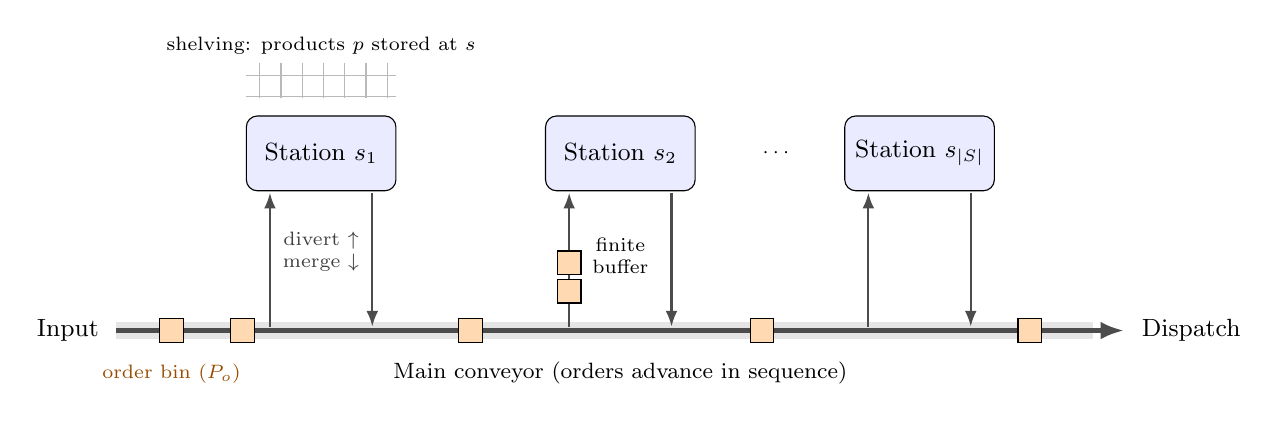
\begin{tikzpicture}[
  font=\small,
  station/.style={draw, rounded corners, fill=blue!8, minimum width=1.9cm, minimum height=0.95cm, align=center},
  bin/.style={draw, fill=orange!30, minimum size=0.30cm, inner sep=0pt},
  conv/.style={line width=2pt, -{Latex[length=3mm]}, black!70},
  spur/.style={thick, -{Latex[length=2mm]}, gray!60!black},
]
% Main conveyor
\draw[line width=6pt, gray!20] (-0.2,0) -- (12.2,0);
\draw[conv] (-0.2,0) -- (12.6,0);
\node[left] at (-0.3,0) {Input};
\node[right] at (12.7,0) {Dispatch};
\node[below, font=\footnotesize] at (6.2,-0.28) {Main conveyor (orders advance in sequence)};

% Stations
\node[station] (s1) at (2.4,2.25) {Station $s_1$};
\node[station] (s2) at (6.2,2.25) {Station $s_2$};
\node[station] (s3) at (10.0,2.25) {Station $s_{|S|}$};
\node[font=\scriptsize] at (8.2,2.25) {$\cdots$};

% Spurs: divert up (left) and merge down (right) for each station
\foreach \x in {2.4,6.2,10.0}{
  \draw[spur] (\x-0.65,0.05) -- (\x-0.65,1.75);
  \draw[spur] (\x+0.65,1.75) -- (\x+0.65,0.05);
}
\node[font=\scriptsize, gray!50!black, align=center] at (2.4,1.0) {divert $\uparrow$\\ merge $\downarrow$};

% Bins flowing on the conveyor
\foreach \x in {0.5,1.4,4.3,8.0,11.4}{ \node[bin] at (\x,0) {}; }
\node[font=\scriptsize, orange!60!black] at (0.5,-0.55) {order bin ($P_o$)};

% Finite buffer (queue) at station s_3
\node[bin] at (5.55,0.5) {};
\node[bin] at (5.55,0.86) {};
\node[align=center, font=\scriptsize] at (6.2,0.95) {finite\\ buffer};

% Shelving (products) at station s_1
\draw[step=0.27cm, gray!55, thin] (1.45,2.95) grid (3.35,3.4);
\node[font=\scriptsize] at (2.4,3.62) {shelving: products $p$ stored at $s$};
\end{tikzpicture}
\caption{Schematic of a pick-and-pass conveyor picking section. Order bins advance along the main conveyor and \emph{divert} onto a station's spur whenever that station stores one of the order's products ($P_o$), are processed, then \emph{merge} back; each diversion is one \emph{station visit}. Concentrating co-ordered products at a shared station reduces the number of visits and the occupancy of each station's finite buffer, the queue whose overflow blocks the main line.}
\label{fig:pickpass_schematic}
\end{figure}

The system is organized around a main conveyor along which orders advance in sequence. Branch lines off the main conveyor correspond to individual picking stations $(S)$. At each station $(s \in S)$, an order ($o \in O$) temporarily leaves the main conveyor so that human pickers can retrieve the required items from nearby shelving and place them into the order bin. After the station’s items are collected, the bin returns to the main conveyor and proceeds on its journey. This process repeats at subsequent stations until all items in the order $(P_o)$ are collected. Finally, the completed bin exits through the main conveyor output, ready for dispatch.

\paragraph{\textbf{Products, orders, and station visits.}} We make the product--order relationship precise. The catalog is the product set $P$ (each element a distinct SKU); $O$ is the set of customer orders observed over the planning horizon. An order $o \in O$ generally requests \emph{several} products, collected in its line set $P_o \subseteq P$; conversely, the \emph{same} SKU typically appears in many different orders, and a product's demand $L_p$ is precisely the number of order-lines (across all orders) in which it occurs. A \emph{station visit} (equivalently a \emph{station stop}) is a single diversion of an order bin onto a station's spur: order $o$ visits station $s$ if and only if at least one product of $P_o$ is stored at $s$. The total objective $\sum_{o}\sum_{s} z_{os}$ therefore counts, across all orders, the number of distinct stations each order must stop at; an \emph{order split} occurs whenever an order's products are spread across more than one station, forcing more than one visit. Because each product is assigned to exactly one station, concentrating co-ordered products at a shared station is what reduces visits. We assign each product to a single station for operational simplicity and to avoid duplicating inventory and replenishment effort across zones; relaxing this to allow high-demand SKUs at multiple stations is a natural extension discussed in \cref{sec:conclusion}.

\subsection{Objective: Minimizing Station Visits}\label{par:minimizing_visits}
While traditional CSLAP models focus on minimizing travel distance, the realities of conveyor-driven systems dictate that the physical stopping of a box is the primary source of operational friction. Consequently, our primary objective is to minimize the total number of station visits per order. This directly increases total warehouse efficiency through two practical dimensions:

\paragraph{\textbf{1. Eliminating Fixed Stopping Overhead: }}
In a real-world automated environment, every time an order bin diverts into a picking station, it incurs a fixed time penalty independent of the number of items actually retrieved. The box must be mechanically inducted, the operator must physically scan its barcode, and the warehouse management system must retrieve and display the required products. By strategically grouping highly correlated items into the same station, an order collects more products in a single stop. Mathematically and practically, a single, slightly extended stop to pick multiple items is significantly more time-efficient than multiple brief stops fragmented across the warehouse.

\paragraph{\textbf{2. Buffer Decongestion via Concentrated Picking: }}
To illustrate the impact on system-level congestion, consider a single picking station with a calibrated daily processing capacity of $1,000$ product lines. The station features a finite physical buffer where incoming boxes queue to be processed. We can fulfill this $1,000$-line workload in two distinct scenarios:
\begin{itemize}
    \item \textit{Fragmented Picking (High Visits):} $500$ distinct orders visit the station, each requiring only $2$ products. This forces $500$ physical boxes into the station's buffer throughout the day.
    \item \textit{Concentrated Picking (Low Visits):} $200$ distinct orders visit the station, each requiring $5$ products. 
\end{itemize}
In the second scenario, the operator accomplishes the exact same amount of productive picking work (1,000 lines), but the station handles 60\% fewer physical boxes. By drastically reducing the physical occupancy of the buffer queue, we prevent local overflows, which would otherwise cause upstream blockages on the main conveyor, ensuring a continuous flow of network traffic.

\subsection{The Hard Constraint: Workload Balancing}\label{par:balanced_workload} 
Aggressively concentrating picks to reduce visits poses a specific systemic risk. A pick-and-pass conveyor functions as a network of interconnected queues \cite{kim2020},\cite{tarczynski2023}. If highly correlated items are clustered too tightly without bounds, the optimization will route an overwhelming majority of warehouse traffic to a single, hyper-correlated station. As the arrival rate of bins approaches that picker's service rate, expected wait times rise sharply, diverging as the utilisation $\rho$ approaches one (scaling as $1/(1-\rho)$ for an M/M/1 queue), ultimately leading to starvation at other stations and total network blocking.

To structurally prevent this outcome, "workload balancing" must act as a hard mathematical constraint. In our formulation, we explicitly bound the daily utilization distribution to stay strictly within each station's pre-established maximum capacity ($T_s$). Minimizing station visits under this rigid limit guarantees that we achieve the aforementioned buffering and overhead benefits without inadvertently creating localized bottlenecks.

\subsection{Modeling Abstraction}
To translate these dynamics into a tractable mathematical formulation, we model CSLAP at the station level rather than at the level of individual storage slots. We make the practical assumption that each station’s internal shelving is \emph{modular}: dividers can be rearranged without altering the station’s \emph{total} storage capacity. This intra-station flexibility allows us to concentrate on the fundamental decision, \emph{which products $(p \in P)$ should share the same station}, without being restricted by fixed slot geometries. Throughout our analysis, the global physical capacity constraint ($\zeta_s$) of each station is strictly respected. For clarity we model each product as occupying one unit of a station's location budget $\zeta_s$; heterogeneous product footprints can be incorporated without structural change by replacing the unit count in Constraint~\eqref{con15} with a per-product size $g_p$ (i.e. $\sum_{p} g_p x_{ps} \le \zeta_s$), which we leave to the size-aware extension noted in \cref{sec:conclusion}.


\begin{table}[H]
\centering
\small 
\begin{tabular}{cl}
\toprule
\textbf{Symbol} & \textbf{Definition}\\
\midrule
$P, O, S$ & Sets of products, orders, and stations\\
$P_o$ & Set of products requested in order $o \in O$\\
$\zeta_s$ & Number of available storage locations at station $s \in S$\\
$L_p$ & Average daily number of pick-lines for product $p \in P$ (lines/day)\\
$V_s$ & Processing speed at station $s \in S$ (lines/day)\\
$T_s$ & Maximum daily time capacity allocated to station $s$ (fraction of a day)\\
$K_s$ & Set of feasible patterns (product assignments) for station $s \in S$\\
\bottomrule
\end{tabular}
\caption*{Summary of key notations}
\label{tab:notation}
\end{table}




\section{Mathematical Model}\label{sec:LP_Approach}

To structurally and formally address the Correlated Storage Location Assignment Problem (CSLAP) in an automated context, we formulate it as a Mixed-Integer Linear Programming (MILP) model. This complete formulation simultaneously minimises station visits and enforces strict, balanced workloads. Building on the demand-correlation ideas of \citet{wang2020}, who focused on minimizing travel distance, we fundamentally redirected the objective toward minimizing the \emph{number of station stops}. Orders thus flow through fewer stations, systematically cutting mechanical queueing and handling time.

The formulation employs binary decision variables to encode product–station assignments and auxiliary variables to record, for each order, the stations it visits. The formulation ensures capacity constraints, workload balancing, and station visit counting, which is internally consistent with the corresponding product-to-station assignments.

%\noindent \textbf{Model Formulation}


\noindent \textbf{Decision variables:}
\begin{itemize}
    \item $x_{ps}$: Binary variable indicating whether product $p \in P$ is assigned to station $s \in S$.
    \item $z_{os}$: Auxiliary variable indicating whether order $o \in O$ needs to visit station $s \in S$ (completely dependent on $x_{ps}$). 

\end{itemize}

\noindent \textbf{Objective function:}

\begin{equation}
\min \sum_{o \in O} \sum_{s \in S} z_{os}
\label{obj}
\end{equation}
The objective is to minimize the total number of station visits required across all orders.

\noindent \textbf{Constraints:}

\begin{align}
&\sum_{s \in S} x_{ps} = 1 \quad \forall p \in P \label{con14}\\
&\sum_{p \in P} x_{ps} \leq \zeta_s \quad \forall s \in S \label{con15}\\
&x_{ps} \leq z_{os} \quad \forall p \in P_o, \forall o \in O, \forall s \in S \label{con16}\\
&\sum_{p \in P} x_{ps} \cdot \frac{L_p}{V_s} \leq T_s \quad \forall s \in S \label{con17}\\
&x_{ps} \in \{0, 1\}, \quad z_{os} \in [0,1], \quad \forall p \in P, o \in O, s \in S 
\end{align}
\\
\noindent Here, Constraint \eqref{con14} ensures each product is assigned to exactly one station, while Constraint \eqref{con15} respects the physical capacity limit of each station. Constraint \eqref{con16} ensures $z_{os}$ is mapped exactly to the visits (acting as a logical OR without needing a native Big-M formulation since the objective natively minimizes $\sum z_{os}$). Finally, Constraint \eqref{con17} enforces a balanced workload on each station.

\section{Solution Methods}\label{sec:methodology}

Having established the mathematical model, we now present the methods used to solve it at scale, mirroring the three operational roles set out in the introduction: a set-variable reformulation amenable to a hybrid local-search engine (strategic optimization), a fast greedy clustering heuristic (operational agility), and a set-partitioning Column Generation framework (structural decomposition). These are subsequently benchmarked against the classic meta-heuristics described in \cref{sec:meta_benchmarking}.

\subsection{Strategic Optimization: Set-Variable MILP Reformulation}\label{sec:set_reformulation}
To solve the mathematical model efficiently, the problem can be reformulated using \emph{set decision variables} rather than standard binary or continuous variables \cite{blaisemodeling}. When utilizing Hexaly's local-search solver engine, a set decision variable acts as a single, high-level entity representing an unordered subset of a finite domain. In this formulation, we create one such variable \( \Phi_s \) for every pick-station $s \in S$; its value is the subset of product indices assigned to that station. Consequently, the standard binary matrix $x_{ps}$ is replaced by the compact family \( \{\Phi_s\}_{s \in S} \). This shift reduces the number of declared decision variables from $|P| \times |S|$ to $|S|$ sets. The reduction concerns the representation, not the underlying combinatorial complexity: the model still encodes which of the $|P|$ products goes to which of the $|S|$ stations, and the assignment problem remains NP-hard \cite{garey1979computers}. Its value is operational. By exposing high-level operators (\textit{partition}, \textit{contains}, and \textit{count}) and a compact move space, the set representation lets the local-search engine navigate the flat, step-function landscape more effectively than by flipping $|P|\times|S|$ individual binary flags.

\subsection{Operational Agility: Greedy Clustering Heuristic}
\label{sec:heuristic_clustering}

Because the exact MILP formulation becomes computationally intractable for large-scale, industrial-sized warehouse instances, we developed a fast heuristic approach. This method bridges the gap between computational feasibility and operational quality by partitioning the product set into tightly bound ``communities'' of highly correlated items and sequentially assigning them to physical picking stations.

Our method draws foundational inspiration from agglomerative clustering techniques previously established in the CSLAP literature. For instance, \cite{chuang2016} successfully utilized Between-Item Association (BIA) to iteratively merge highly correlated items into hierarchical clusters, ultimately assigning them closer to depots to minimize manual travel distance. We adapt and significantly extend this pair-wise logic for the automated conveyor paradigm. Rather than assigning clusters based on proximity to a depot, our heuristic relies on greedy graph-connectivity principles \cite{west2001introduction} to build disjoint product communities.

Furthermore, our approach fundamentally diverges from traditional unconstrained clustering by introducing dynamic, scale-relative boundary parameters. Fixed clustering thresholds inherently fail when bridging problem magnitudes; a co-occurrence count that represents strong affinity in a 50-SKU catalog may be statistically indistinguishable from random noise in a 20,000-SKU environment. By utilizing dynamically scaled thresholds, we ensure that the generated communities remain robust across varying scales while strictly respecting the physical and temporal capacity limits of heterogeneous automated stations.

Let $N = |P|$ be the total number of products. The heuristic requires no per-instance tuning: it fixes a small set of scale-relative constants ($1/100$, $1/50$, $\mathrm{RATIO\_TO\_KEEP}=0.1$, and the $5$--$15$ bounds on $\mathrm{MNOPPC}$), each chosen so that the corresponding threshold tracks a fixed fraction of catalog volume, and derives the operative thresholds as functions of $N$. Feasibility is governed by the station capacity $\zeta_s$ rather than by these correlation thresholds, to which the output is robust under moderate variation. The thresholds are:



\begin{itemize}
    \item \(\mathrm{MIN\_FREQ\_PREPROC} = \max(2, \lfloor N / 100 \rfloor)\): The minimum order frequency for a product to be considered. Anchoring this to exactly 1\% of the catalog filters out scale-relative noise, with a strict floor of 2 to eliminate single-occurrence anomalies.
    \item \(\mathrm{MIN\_FREQ} = \max(2, \lfloor N / 50 \rfloor)\): The absolute minimum co-occurrence count for a product pair. Scaling this to 2\% of the dataset guarantees that candidate pairs represent a mathematically significant correlation relative to the total warehouse volume.
    \item \(\mathrm{RATIO\_TO\_KEEP} = 0.1\): A constant fractional edge. A pair is retained only if their co-occurrence constitutes at least 10\% of a given product's total historical demand.
    \item \(\mathrm{MNOPPC} = \max(5, \min(15, \lfloor N / 20 \rfloor))\): The maximum number of products allowed in a single community. This scales proportionally to 5\% of the catalog but is artificially bounded between 5 and 15 items to respect the physical geometry of automated picking zones and prevent the formation of operationally infeasible "mega-clusters."
\end{itemize}

\paragraph{Algorithmic Phasing:}
By addressing the dimensional complexities inherent in CSLAP computationally, this dynamic scaling provides a generalized framework that requires no manual parameter tuning. The core logic proceeds in four sequential phases, visually summarized in \cref{fig:heuristic_flowchart}. (The formal, step-by-step procedural pseudocode is provided in \ref{sec:appendix_heuristic}).

\begin{enumerate}
    \item \textbf{Preprocessing:} We filter out low-frequency noise and generate a sorted list of highly correlated product pairs %that survive the dynamic thresholds.
    \item \textbf{Community Formation:} Using a greedy expansion strategy, we iteratively build disjoint item communities. Starting with the strongest pair, we absorb the next most correlated products until the physical capacity limit ($\mathrm{MNOPPC}$) is reached.
    \item \textbf{Post-Processing:} Any residual or low-frequency products are swept and inserted into the most highly correlated available communities with remaining capacity.
    \item \textbf{Station Assignment:} Communities are ranked by cumulative demand and assigned to physical stations based on majority historical preference, strictly enforcing the station's physical capacity ($\zeta_s$). If an entire community cannot fit, it is split intelligently to preserve high-correlation links.
\end{enumerate}

\vspace{0.5cm}

\begin{figure}[H]
\centering
\resizebox{0.95\linewidth}{!}{%
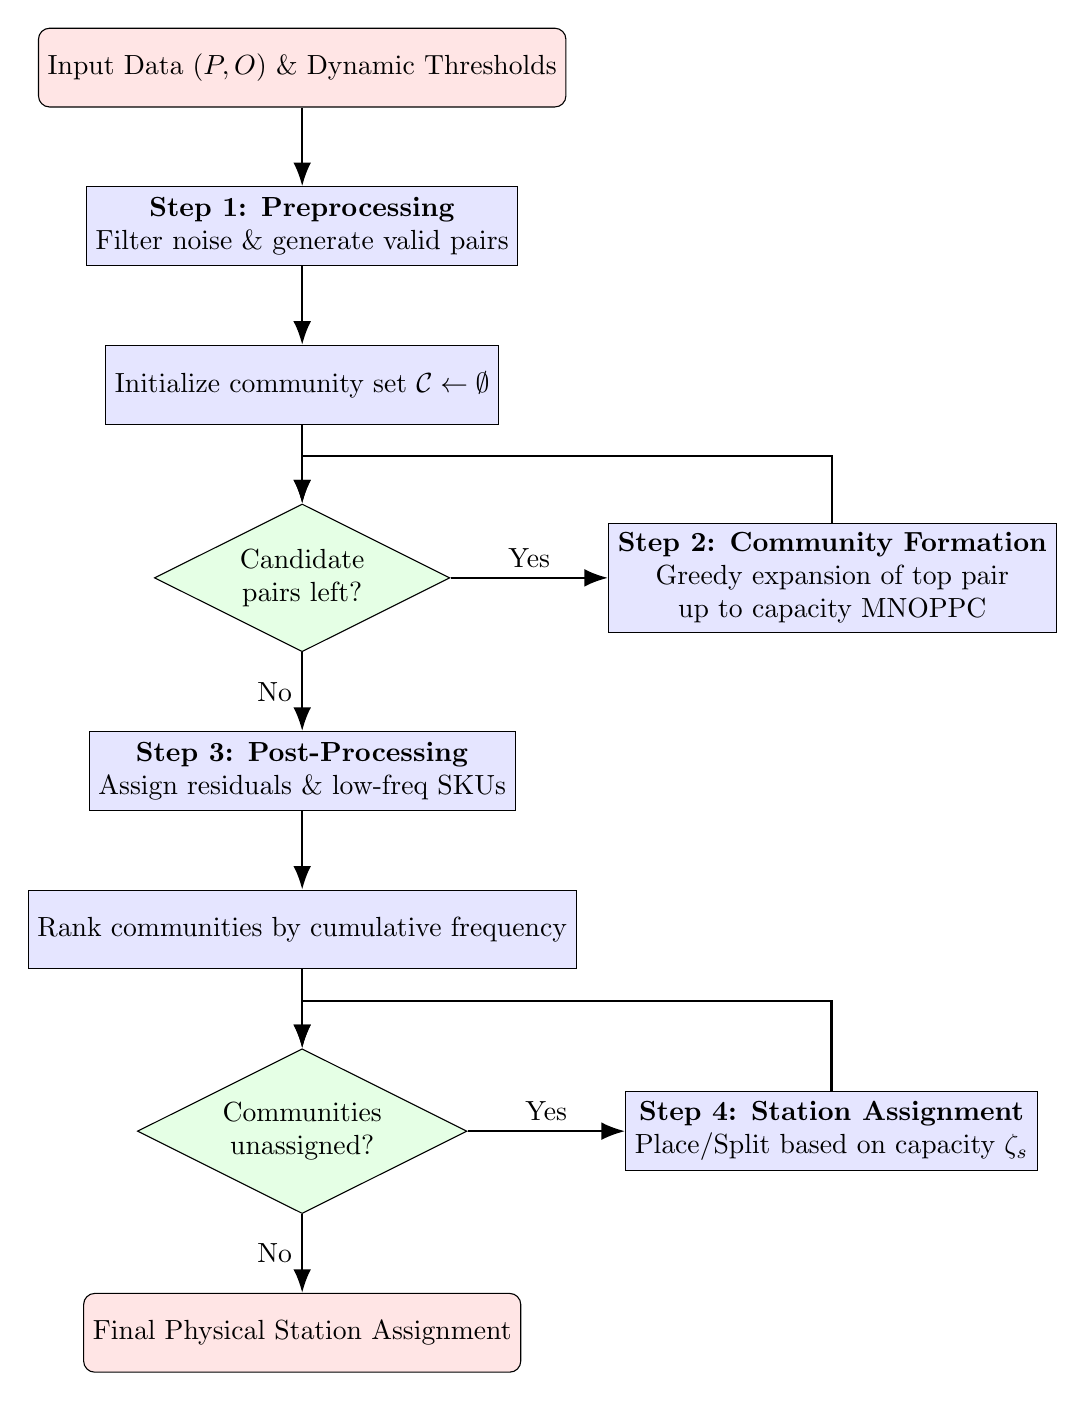
\begin{tikzpicture}[
    node distance=1.2cm and 1.5cm,
    startstop/.style={rectangle, rounded corners, minimum width=3.5cm, minimum height=1cm, text centered, draw=black, fill=red!10},
    process/.style={rectangle, minimum width=4cm, minimum height=1cm, text centered, draw=black, fill=blue!10, align=center},
    decision/.style={diamond, aspect=2, minimum width=3.5cm, minimum height=1cm, text centered, draw=black, fill=green!10, align=center},
    arrow/.style={thick, -{Latex[length=3mm]}}
]

% Nodes
\node (start) [startstop] {Input Data ($P, O$) \& Dynamic Thresholds};

\node (preproc) [process, below=1cm of start] {\textbf{Step 1: Preprocessing}\\Filter noise \& generate valid pairs};

\node (initcomm) [process, below=1cm of preproc] {Initialize community set $\mathcal{C} \leftarrow \emptyset$};

\node (decide1) [decision, below=1cm of initcomm] {Candidate\\pairs left?};

\node (form) [process, right=2cm of decide1] {\textbf{Step 2: Community Formation}\\Greedy expansion of top pair\\up to capacity MNOPPC};

\node (post) [process, below=1cm of decide1] {\textbf{Step 3: Post-Processing}\\Assign residuals \& low-freq SKUs};

\node (sort) [process, below=1cm of post] {Rank communities by cumulative frequency};

\node (decide2) [decision, below=1cm of sort] {Communities\\unassigned?};

\node (assign) [process, right=2cm of decide2] {\textbf{Step 4: Station Assignment}\\Place/Split based on capacity $\zeta_s$};

\node (end) [startstop, below=1cm of decide2] {Final Physical Station Assignment};

% Arrows
\draw [arrow] (start) -- (preproc);
\draw [arrow] (preproc) -- (initcomm);
\draw [arrow] (initcomm) -- (decide1);
\draw [arrow] (decide1) -- node[anchor=south] {Yes} (form);
\draw [arrow] (form) |- ($(initcomm.south) + (0,-0.4)$) -| (decide1);
\draw [arrow] (decide1) -- node[anchor=east] {No} (post);
\draw [arrow] (post) -- (sort);
\draw [arrow] (sort) -- (decide2);
\draw [arrow] (decide2) -- node[anchor=south] {Yes} (assign);
\draw [arrow] (assign) |- ($(sort.south) + (0,-0.4)$) -| (decide2);
\draw [arrow] (decide2) -- node[anchor=east] {No} (end);

\end{tikzpicture}
}
\caption{Logical flowchart of the Greedy Product Clustering and Station Assignment heuristic.}
\label{fig:heuristic_flowchart}
\end{figure}

\noindent This heuristic approach offers a favorable balance between computational speed and solution quality. By aggressively addressing the dimensional complexities inherent in CSLAP, it provides a scalable framework capable of adapting to evolving order patterns and automated warehouse configurations in near-real-time, at the price of treating the workload cap as a soft target (\cref{sec:numerical_results}).



\subsection{Structural Decomposition: Set-Partitioning Column Generation}\label{sec:cg}

The heuristic of \cref{sec:heuristic_clustering} returns fast layouts but no certificate, and the set-variable MILP of \cref{sec:set_reformulation} carries no valid bound on the visit count. We close this gap with a column generation framework built on a set-partitioning decomposition of the model of \cref{sec:LP_Approach}. Column generation solves programs over very large column sets by pricing variables on demand \cite{lubbecke2005selected}, and it is well matched to the set-covering and set-partitioning structure that recurs in logistics and scheduling \cite{desrochers1989column, muter2022}. We first state the general, station-indexed master, which handles heterogeneous stations and is the formulation we deploy on the industrial instance of \cref{sec:numerical_results}; we then derive the aggregated, station-agnostic reformulation that we use on the homogeneous synthetic family, where it eliminates the symmetry the general master carries.

\subsubsection{A Station-Indexed Set-Partitioning Master}\label{sec:cg_master_general}

CSLAP decomposes naturally by station. Recall from the notation of \cref{sec:problem_definition} that $K_s$ denotes the family of feasible patterns for station $s$: subsets $q \subseteq P$ with $|q| \le \zeta_s$ and $\sum_{p \in q} L_p / V_s \le T_s$. Let $U$ be the set of \emph{distinct} multi-item order supports, each carrying a multiplicity weight $w_u$ equal to the number of orders that share that support; aggregating orders into weighted distinct supports keeps the raw order count out of the master. With one column per station--pattern pair and the aggregated cost $c_q = \sum_{u \in U} w_u\,\mathbf{1}[q \cap u \neq \emptyset]$ counting the weighted supports a pattern touches, the master problem reads
\[
\min_{x}\ \sum_{s \in S} \sum_{q \in K_s} c_q\, x_{sq}
\]
\begin{align}
& \sum_{s \in S} \sum_{q \in K_s:\, p \in q} x_{sq} \ge 1 \qquad (\sigma_p \ge 0) \quad \forall p \in P, \label{cg:cover_gen}\\
& \sum_{q \in K_s} x_{sq} \le 1 \qquad (\mu_s \le 0) \quad \forall s \in S, \label{cg:conv_gen}\\
& 0 \le x_{sq} \le 1 \quad \forall s \in S,\ q \in K_s. \nonumber
\end{align}
Constraint \eqref{cg:cover_gen} covers every product, and the per-station convexity rows \eqref{cg:conv_gen} select at most one pattern per station; for any integer solution whose patterns partition the catalog the objective equals the total station visits of the multi-item orders exactly, singleton orders contributing a constant. This is the conventional Dantzig--Wolfe shape for our assignment model \cite{lubbecke2005selected, desrochers1989column}: pattern feasibility is delegated to $|S|$ pricing subproblems, one per station, each minimizing the reduced cost $c_q - \sum_{p \in q} \sigma_p - \mu_s$ over the patterns satisfying that station's two resource limits, $\sum_p a_p \le \zeta_s$ and $\sum_p L_p\, a_p \le T_s V_s$. Because the pricing constraint matrix is identical across stations up to these two right-hand sides, a single persistent pricing model can serve every station, each call swapping only two values; a full pricing pass at one dual vector then yields the per-station Farley-type bound $\mathrm{LB} = z_{\mathrm{RMP}} + \sum_{s \in S} \min(0,\ \mathrm{rc}^{\mathrm{lb}}_s)$ developed in \cref{sec:cg_bound}. This station-indexed master is exactly the formulation we run on the heterogeneous industrial instance in \cref{sec:numerical_results}.

For a \emph{homogeneous} warehouse, however, the station index carries no information and becomes a computational liability. When every station shares one slot capacity $\zeta$, one speed $V$ and one workload cap $T$, the pattern families $K_s$ coincide and the master is invariant under permutations of the station labels: the relaxation is massively degenerate, and integer search revisits relabeled copies of the same partition \cite{vanderbeck2000dw}. The multiplicity of the pricing subproblems is equally redundant, since all $|S|$ calls solve the same model at the same duals up to $\mu_s$. The aggregated reformulation below removes both burdens by construction rather than managing them at run time.

\subsubsection{Aggregated Reformulation for Homogeneous Warehouses}\label{sec:cg_master_agg}

Consider the homogeneous case with capacity tight, $|P| = |S|\cdot\zeta$. CSLAP is then exactly a cardinality-constrained set-partitioning problem over \emph{station-agnostic} product bundles: partition the catalogue into at most $|S|$ bundles of at most $\zeta$ products, and the number of stations an order visits equals the number of selected bundles its line set touches. A column then needs no station index. Let $Q$ be the family of feasible bundles; over the current pool $Q' \subseteq Q$ the restricted master problem (RMP) reads
\[
\min_{x}\ \sum_{q \in Q'} c_q\, x_q, \qquad c_q = \sum_{u \in U} w_u\,\mathbf{1}[q \cap u \neq \emptyset],
\]
\begin{align}
& \sum_{q \ni p} x_q \ge 1 \qquad (\sigma_p \ge 0) \quad \forall p \in P, \label{cg:cover}\\
& \sum_{q \in Q'} x_q \le |S| \qquad (\mu \le 0), \label{cg:card}\\
& 0 \le x_q \le 1 \quad \forall q \in Q'. \nonumber
\end{align}
As before, the master objective equals the total station visits of the multi-item orders exactly for any partition. Unlike the station-indexed master of \cref{sec:cg_master_general}, whose $|S|$ convexity rows \eqref{cg:conv_gen} distinguish interchangeable stations, the single cardinality row \eqref{cg:card} condenses the allocation decision into one constraint and yields the single dual $\mu$, structurally eliminating the per-station symmetry together with the per-station multiplicity of the pricing subproblems. At integrality under tight capacity the covering rows act as an exact partition into $|S|$ full bundles, so the relaxation and its integer counterpart carry the same combinatorial meaning. Where capacity is slack, the covering inequality together with the visit-minimizing objective still returns an exactly-once assignment, since the objective never benefits from placing a product in more than one bundle.


\subsubsection{Pricing Subproblem}

A single pricing subproblem generates improving bundles. With $a_p \in \{0,1\}$ marking the products of a candidate bundle and $z_u \in [0,1]$ marking the supports it touches, the most negative reduced cost solves
\[
\min\ \sum_{u \in U} w_u\, z_u - \sum_{p \in P} \sigma_p\, a_p - \mu
\]
\begin{align}
    & z_u \ge a_p \quad \forall u \in U,\ p \in u, \nonumber\\
    & \sum_{p \in P} a_p \le \zeta, \qquad \sum_{p \in P} \frac{L_p}{V}\, a_p \le T, \nonumber\\
    & a_p \in \{0,1\}, \quad z_u \in [0,1]. \nonumber
\end{align}
The constraint matrix does not depend on the duals, so the pricing MILP is constructed once per instance and each pricing call rewrites only the objective coefficients of the $a_p$ variables on a persistent model; the constant $-\mu$ touches no variable coefficient and is accounted for outside the solve. This is what keeps exact pricing affordable at up to roughly $66{,}000$ distinct supports on the $2{,}000$-SKU instances: the model build is a single up-front cost of about $21$ seconds, while the first exact solve at $50$ SKUs returns in about $0.2$ seconds. A single pricing family thus replaces the $|S|$ station-indexed pricing calls of \cref{sec:cg_master_general}, and encoding coverage per distinct support rather than per order keeps the subproblem's size independent of the raw order count --- the axis on which a direct per-order implementation of the conventional decomposition scales worst.

\subsubsection{Price-and-Complete Matheuristic}\label{sec:cg_matheuristic}

A cardinality-tight partition master does not advance on isolated columns. With covering rows over all products, one cardinality row and bundles of size at most $\zeta$, a single excellent bundle cannot enter the basis until compatible complements cover the remaining products, so column-at-a-time generation plateaus even while deeply negative reduced-cost columns exist. This is a structural property of cardinality-tight partition masters over a flat, step-function objective, not an implementation artifact, and we address it with a coordination mechanism designed for it: the method is driven as a matheuristic whose generation loop emits coordinated column sets --- full feasible partitions --- guided by exact pricing and equipped with the valid bound of \cref{sec:cg_bound}. Its components are the following.

\begin{enumerate}
    \item \emph{Feasibility warm start.} A longest-processing-time packer sorts products by descending order-line workload and assigns each to the least-loaded station that still has a free slot and residual time capacity, producing a feasible, workload-balanced but correlation-blind partition. This is the same deterministic start seeded to the other exact methods (\cref{sec:warm_start}), so initialization bias is excluded. A swap descent polishes it, and the polished partition, together with randomly mutated feasible variants, seeds the initial column pool.

    \item \emph{Penalized swap descent.} A first-improvement local search over pairs of products in different stations accepts a swap on the exact change in $\text{visits} + \rho\sum_i \max(0,\, W_i - T)$, with $\rho$ set to the total order weight, so a workload violation is never traded away for fewer visits. The change induced by a candidate swap is evaluated incrementally in $\mathcal{O}(\deg(p)+\deg(q))$ from a per-station support-count matrix $\mathrm{cnt}[i][u]$, the number of station-$i$ products contained in support $u$: removing $p$ from station $i$ frees exactly the supports whose count drops to zero, and inserting it into station $j$ costs exactly the supports whose count rises from zero. An accepted swap is applied at once and the scan restarts from the new state; above about $300$ products the partner set is sampled to bound the cost of a pass. The descent runs in three roles, namely warm-start polish, per-iteration repair of a completed partition, and a final polish on the leftover budget.

    \item \emph{Dual-guided greedy pricing.} Before the exact pricer is called, an accelerator considers only products with positive dual $\sigma_p$ and tests two orderings, largest $\sigma_p$ first and largest $\sigma_p$ per unit workload first. It grows a bundle one product at a time under the slot and workload caps, tracks the exact reduced cost after every insertion, and returns the best prefix, the insertion point at which the reduced cost was lowest, rather than the filled bin. Only when this fails to produce a negative reduced-cost column does the exact CPLEX pricer decide the iteration.

    \item \emph{Partition completion.} Each priced bundle is completed into a full feasible partition so that a coordinated set of columns enters the master together. Disjoint priced bundles are placed first; the remaining products then join, heaviest first, the feasible station of maximum co-occurrence affinity, where affinity is the total weight of the product's supports already touched by that station, equivalently the minimum marginal visit cost. The completed partition is refined by the swap descent, and all of its bundles enter the master together. Because each completion is itself a feasible primal layout, the method produces a monotone stream of full feasible solutions. Bundles that break the slot or workload caps never enter the master.

    \item \emph{Integer master and deduplication.} After the generation loop the master is re-solved with binary $x_q$ over the accumulated pool. Because the covering rows permit a product to appear in two selected bundles, an explicit repair assigns each duplicated product to the selected station whose other products share the largest total order weight with it and removes it from the rest; a removal can only lower the visit count. The final layout is re-evaluated on the raw orders, and the better of the integer-master layout and the best incumbent partition is polished by the swap descent for whatever budget remains. Every reported visit count is recomputed on the real order stream and is never read from the model objective.
\end{enumerate}

A single wall-clock budget per instance is split across these stages, with about $8\%$ for the warm-start polish, up to $70\%$ for the generation loop, up to $85\%$ for the integer master, and the remainder for the final polish. The method is implemented on IBM CPLEX through its Python interface, with a deterministic seed and one identical configuration for every instance and every size.

\subsubsection{Lower Bound, Convergence and Scope}\label{sec:cg_bound}

At every iteration the method maintains a Farley-type convexity bound \cite{farley1990note}. In the aggregated master the cardinality row admits $|S|$ selected bundles, so
\[
\mathrm{LB} = z_{\mathrm{RMP}} + |S|\cdot \min\!\big(0,\ \mathrm{rc}_{\mathrm{lb}}\big),
\]
where $\mathrm{rc}_{\mathrm{lb}}$ is the dual (best) bound reported by the pricing MILP, a valid lower bound on the minimum reduced cost; the cardinality dual enters it exactly once, through the constant $-\mu$ that the pricing objective already carries. In the station-indexed master of \cref{sec:cg_master_general} the same argument applies row by row and gives $\mathrm{LB} = z_{\mathrm{RMP}} + \sum_{s \in S} \min(0,\ \mathrm{rc}^{\mathrm{lb}}_s)$ with $\mathrm{rc}^{\mathrm{lb}}_s$ the dual bound of station $s$'s pricing problem, whose objective carries that station's convexity dual $-\mu_s$. The pricing dual bound stays valid even when a pricing call is truncated by its time slice, so $\mathrm{LB}$ is a valid lower bound on the optimum throughout the run; degeneracy of the covering master affects how tight this certificate is, never whether it holds. Convergence, meaning the linear master is priced out, is declared only from an exact pricing solve at the true duals with proven optimality.

Within the budgets reported in \cref{sec:reliability_multiseed} this certificate is informative only at $50$ SKUs, where the mean bound of $3{,}272$ sits below the mean of $7{,}592$ visits, and it is vacuous at $500$ SKUs and above. We therefore present the method as a matheuristic with a valid but currently loose certificate rather than as an exact solver. Dual stabilization is the lever that would tighten the bound, which we return to in \cref{sec:future}.

\paragraph{\textbf{Scope.}} The aggregated reformulation of \cref{sec:cg_master_agg} treats identical stations, which holds by construction for the synthetic family, and this flat-warehouse case remains the reference presentation of the method. On a heterogeneous layout such as Company~A the framework reverts to the station-indexed master of \cref{sec:cg_master_general}, retaining the single persistent pricing model (only the two right-hand sides $\zeta_s$ and $T_s V_s$ vary per call), the price-and-complete drive of \cref{sec:cg_matheuristic}, and the per-station form of the bound above. This configuration is evaluated on Company~A in \cref{sec:numerical_results}.




\section{Data Instance Generation and Experimental Setup}
\label{sec:data_generation}

Before delving into the computational outcomes, this section establishes the rigorous experimental framework required to fairly evaluate our proposed methodologies. To bridge the gap between theoretical optimality and industrial application, we must first construct and validate the testing environments. 

This section details the generation of controlled synthetic instances and mathematically validates their structural realism against the real-world dataset we retrieved from Company A. Furthermore, we outline the deterministic initialization procedures and baseline adaptations necessary to ensure an equitable comparison between our MILP and CG solvers, our clustering heuristic, and established literature meta-heuristics (GA, SA-C). By the end of this section, the reader will understand the operational parameters bounding our datasets, the statistical validity of the testing environments, and the strict mathematical conditions under which the algorithms are benchmarked.

\subsection{Synthetic Data Generation and Validation}

To evaluate our models under controlled conditions, we generated four synthetic datasets ($N \in \{50, 500, 1000, 2000\}$ SKUs) adapted from the ``Common Itemset'' approach by \cite{zhang2019cie}. We retained their core mechanics, a correlation degree of $\theta = 0.7$,  and proportional order volumes, while tailoring the environment specifically for station-visit minimization. To eliminate architectural bias, we modeled a uniformly homogeneous warehouse where all stations possess identical physical capacities ($\zeta_s = \lfloor |P| / |S| \rfloor$) and processing speeds ($V_s = 1$). The maximum daily time capacity ($T_s$) was derived by applying a 10\% operational slack to the average global workload, mathematically guaranteeing that a balanced distribution is feasible.

To ensure these instances accurately mirror operational realities, we benchmarked their structural properties against the empirical Company A dataset. First, the synthetic order size distribution ($U[5, 15]$) successfully captures the true industrial median of 10.0 items. Second, to replicate empirical network sparsity, where only 2.47\% of product combinations ever co-occur, we restricted common itemsets to a narrow subset fraction ($U[0.1, 0.5]$). Finally, we validated the $\theta = 0.7$ correlation factor by evaluating the conditional probabilities of the top 1\% most frequently co-occurring pairs. The resulting synthetic affinity (8.89\%) acts as a rigorously conservative baseline against the industrial reality (14.24\%). This confirms that our synthetic data injects the necessary structural correlation without artificially inflating heuristic performance, ensuring our algorithmic evaluations translate reliably to real-world applications.

\subsection{Deterministic Feasibility Warm Start for Exact Solvers}\label{sec:warm_start}

While our clustering heuristic (\cref{sec:heuristic_clustering}) effectively minimizes station visits, it prioritizes topological item affinities over strict workload boundaries ($T_s$). Seeding exact solvers with such unconstrained outputs causes commercial engines to reject the initial states as mathematically infeasible. To circumvent this, we introduce a deterministic \textit{Feasibility Warm Start}. Temporarily disregarding item correlation, we deploy a Longest Processing Time (LPT) strategy: items are sorted by independent order-line frequency and greedily distributed into the station with the lowest aggregate workload. This mathematically guarantees a starting assignment that strictly satisfies both the physical ($\zeta_s$) and temporal ($T_s$) constraints. Injecting this valid bound accelerates the initial branching process for the MILP and CG frameworks. Seeding all exact models with this identical baseline ensures an equitable computational evaluation, strictly isolating each solver's algorithmic capacity to navigate the solution space and improve upon the exact same initial conditions.



\subsection{Meta-Heuristic Benchmarking and Baseline Adaptations}
\label{sec:meta_benchmarking}

To rigorously validate our exact methodologies, we benchmark them against two classic meta-heuristics established in the CSLAP literature: Simulated Annealing with Correlated Interchange (SA-C) \cite{kim2012, zhang2019cie} and a Genetic Algorithm (GA) \cite{pan2015}. 

Because our primary objective of minimizing discrete station visits per order is inherently a step-function, it generates a flat objective space topology where local item swaps rarely yield immediate objective improvements. To prevent these probabilistically guided searches from stalling on local plateaus, we fundamentally adapted the objective function evaluation for both algorithms. The evaluation integrates the primary visit count with strict capacity and workload penalties, supplemented by a secondary \textit{dispersion tie-breaking penalty}. This secondary metric mathematically penalizes the spatial spread of highly correlated items, guiding the search toward promising neighborhoods even when the primary metric remains temporarily static.

Algorithmically, the SA-C implementation navigates this search space using a correlated interchange operator, which specifically groups and swaps frequently co-occurring SKU pairs under a geometric decay parameter for probabilistic acceptance. Conversely, the GA baseline maintains a pool of candidate solution vectors, iteratively generating new assignments via quality-proportional selection, random perturbation (swap) operators, and subset exchange mechanisms (adapted from the Partially Mapped Crossover logic) for discrete station-assignments. The GA also incorporates a strict post-exchange capacity-repair mechanism, reallocating items from overfull to underfull stations to maintain physical feasibility in every iteration.

Finally, to ensure a strictly equitable computational comparison, we standardized the initialization process. While SA-C and GA natively utilize Cube-per-Order Index (COI) and capacity-feasible random initializations respectively, we explicitly seed both algorithms with the exact same starting solutions provided to our mathematical solvers (the deterministic LPT assignment for synthetic instances, and the legacy layout for the industrial case study). This guaranteed standardization ensures that any divergence in final solution quality strictly isolates the algorithmic capacity of exact mathematical bounding versus heuristic search, removing initialization bias.


% =======================================================
% SECTION 5: NUMERICAL RESULTS
% =======================================================
\section{Numerical Results and Managerial Insights}
\label{sec:numerical_results}

Building upon the rigorously defined experimental setup, this section presents the comprehensive computational evaluation of our proposed methodologies and distills the resulting managerial insights. The analysis is structured to progressively scale from the generated synthetic datasets, to the real-world industrial dataset. 

We first present the synthetic benchmarking results to establish the computational scalability limits of traditional solvers and to demonstrate the mathematical superiority of our set-variable MILP against literature baselines. We then transition to the 21,874-SKU (stock-keeping units) industrial case study to validate the performance of our approaches in this real-world scenario. Finally, we validate the operational robustness of our best solution approach via temporal hold-out testing and demonstrate a restricted-reassignment model. By the end of this section, the reader will understand the precise computational trade-offs of each algorithm and how warehouse managers can deploy these exact tools to achieve continuous, non-disruptive throughput improvements.

\subsection{Benchmarking on Synthetic Data}\label{sec:reliability_multiseed}
The set-variable MILP (Hexaly), GA, SA-C and the greedy heuristic all rely on randomised search, so a single run cannot establish whether a ranking reflects method quality or one favourable draw. We evaluate every method over multiple, independently generated instances per size, drawn from the same Zhang common-itemset generator with distinct seeds, and report the mean station-visit count with a $95\%$ confidence interval (CI) together with paired significance tests. The four scales carry $50$, $500$, $1{,}000$ and $2{,}000$ SKUs; the station counts and the mean order volumes are listed in the gray band above each block of \cref{tab:exp02a_reliability}. The set-variable MILP serves as the per-instance reference: each method's gap is measured against the strongest solution obtained on the same instance rather than against the best of the heuristic pool.

All optimizing methods run under a common per-size wall-clock budget, reported in the Time column of \cref{tab:exp02a_reliability}: $120/300/600/1{,}200$\,s across the four sizes. The set-variable MILP and the aggregated set-partitioning column generation of \cref{sec:cg} each consume the full budget at every size, so their visit comparison is made at equal computational effort. GA and SA-C run under the same budget and may stop earlier when their own schedules complete, as at $50$ and $2{,}000$ SKUs; a run may finish inside the budget but never exceeds it. The greedy heuristic has no time parameter and runs to completion well within the budget, and the Feasible Start (LPT) seed is immediate. Every ranking below is therefore read at this shared budget rather than at method-specific times.

\begin{table}[H]
  \centering
  \footnotesize\setlength{\tabcolsep}{3pt}
  \begin{threeparttable}
  \begin{tabularx}{\linewidth}{@{}l*5{>{\centering\arraybackslash}X}@{}}
    \toprule
    \textbf{Method} & \textbf{Mean Visits} & \textbf{95\% CI} & \textbf{Gap to MILP} & \textbf{Time (s)} & \textbf{WL-viol.\ inst.} \\
    \midrule
    \multicolumn{6}{l}{\cellcolor{gray!15}\textbf{Scale: 50 SKUs} $\mid$ Stations: 5 $\mid$ Mean orders: 2,036 $\mid$ $K{=}12$ $\mid$ Budgets: 120\,s} \\
    \midrule
    \textbf{MILP (set-var.)}\tnote{b} & \textbf{7,557} & [6,828, 8,286] & (ref) & 120 & 0\% \\
    CG (set-part.)    & 7,592 & [6,860, 8,323] & $+0.5\%$ & 120 & 0\% \\
    SA-C                     & 7,657 & [6,914, 8,399] & $+1.3\%$ & 39 & 0\% \\
    Heuristic                & 7,700 & [6,964, 8,437] & $+2.0\%$ & 1 & 100\% \\
    GA                       & 7,767 & [7,022, 8,513] & $+2.8\%$ & 34 & 0\% \\
    Feasible Start (LPT)\tnote{c} & 8,857 & [8,054, 9,661] & $+17.4\%$ & $<0.1$ & 0\% \\
    \midrule
    \multicolumn{6}{l}{\cellcolor{gray!15}\textbf{Scale: 500 SKUs} $\mid$ Stations: 5 $\mid$ Mean orders: 20,832 $\mid$ $K{=}10$ $\mid$ Budgets: 300\,s} \\
    \midrule
    \textbf{MILP (set-var.)}\tnote{b} & \textbf{76,041} & [68,118, 83,964] & (ref) & 300 & 0\% \\
    CG (set-part.)    & 76,624 & [68,568, 84,680] & $+0.8\%$ & 300 & 0\% \\
    Heuristic                & 78,655 & [70,515, 86,795] & $+3.5\%$ & 9 & 80\% \\
    GA                       & 84,417 & [75,359, 93,475] & $+11.0\%$ & 300 & 0\% \\
    SA-C                     & 88,372 & [78,937, 97,808] & $+16.2\%$ & 300 & 0\% \\
    Feasible Start (LPT)\tnote{c} & 90,177 & [80,419, 99,936] & $+18.5\%$ & $<0.1$ & 0\% \\
    \midrule
    \multicolumn{6}{l}{\cellcolor{gray!15}\textbf{Scale: 1,000 SKUs} $\mid$ Stations: 10 $\mid$ Mean orders: 38,743 $\mid$ $K{=}4$ $\mid$ Budgets: 600\,s} \\
    \midrule
    CG (set-part.)    & 192,288 & [149,062, 235,513] & $-0.1\%$ & 600 & 0\% \\
    \textbf{MILP (set-var.)}\tnote{b} & \textbf{192,330} & [150,290, 234,370] & (ref) & 600 & 0\% \\
    Heuristic                & 196,155 & [151,570, 240,740] & $+1.9\%$ & 19 & 100\% \\
    GA                       & 232,543 & [182,649, 282,437] & $+21.0\%$ & 600 & 0\% \\
    SA-C                     & 241,451 & [195,307, 287,594] & $+25.8\%$ & 600 & 25\% \\
    Feasible Start (LPT)\tnote{c} & 245,228 & [195,489, 294,967] & $+27.7\%$ & $<0.1$ & 0\% \\
    \midrule
    \multicolumn{6}{l}{\cellcolor{gray!15}\textbf{Scale: 2,000 SKUs}\tnote{a} $\mid$ Stations: 20 $\mid$ Mean orders: 78,698 $\mid$ $K{=}3$ $\mid$ Budgets: 1,200\,s} \\
    \midrule
    CG (set-part.)    & 475,035 & [405,554, 558,724] & $-2.4\%$ & 1,200 & 0\% \\
    Heuristic                & 483,131 & [411,517, 565,068] & $-0.8\%$ & 38 & 100\% \\
    \textbf{MILP (set-var.)}\tnote{b} & \textbf{486,972} & [410,917, 568,247] & (ref) & 1,200 & 0\% \\
    GA                       & 608,269 & [520,733, 731,940] & $+24.8\%$ & 909 & 0\% \\
    SA-C                     & 614,094 & [528,037, 737,715] & $+26.0\%$ & 1,096 & 0\% \\
    Feasible Start (LPT)\tnote{c} & 621,096 & [533,942, 748,257] & $+27.4\%$ & $<0.1$ & 0\% \\
    \bottomrule
  \end{tabularx}
  \begin{tablenotes}\footnotesize
    \item[a] At $K{=}3$ the $t$-interval is uninformative; the bracket reports the observed [min, max] range, not a CI.
    \item[b] Set-variable MILP of \cref{sec:set_reformulation} (solved with Hexaly), used as the per-instance reference; ``Gap to MILP'' is the mean per-instance excess visits over this reference. ``WL-viol.\ inst.'' is the fraction of instances breaching the workload cap; a method is operationally feasible only at $0\%$. CG (set-part.) is the aggregated set-partitioning column generation of \cref{sec:cg} (solved with CPLEX).
    \item[c] Feasible Start (LPT): the shared deterministic LPT seed handed to every method, shown as a correlation-blind anchor and excluded from the method-ranking claims. ``Time (s)'' is the wall-clock time under the common per-size budget, equal to that budget for methods that consume it fully; ``Mean orders'' is the mean order count across the $K$ instances of the block.
  \end{tablenotes}
  \end{threeparttable}
  \caption{Multi-instance benchmark across the synthetic instance distribution, with the set-variable MILP as the per-instance reference. Rows within each scale block are sorted by ascending mean visits, with the Feasible Start (LPT) anchor placed last. Mean station visits with $95\%$ CI, mean gap to the reference, solve time under the common per-size budget, and the fraction of instances breaching the workload cap.}
  \label{tab:exp02a_reliability}
\end{table}

Three conclusions hold across the random draws; a fourth, on the column generation, follows below. First, among the greedy heuristic and the literature meta-heuristics, the \textbf{set-variable MILP is the best feasible method at every scale}, and its margin over the literature baselines widens with problem size: GA and SA-C trail it by $2.8\%$ and $1.3\%$ at $50$ SKUs, but by $24.8\%$ and $26.0\%$ at $2{,}000$ SKUs. These gaps are statistically robust. A paired Wilcoxon signed-rank test separates the MILP from both GA and SA-C at $50$ and $500$ SKUs ($p=4.9\times10^{-4}$ and $p=1.95\times10^{-3}$ respectively), and at $1{,}000$ and $2{,}000$ SKUs the paired $t$-test confirms the same ordering (the Wilcoxon test is underpowered at $K=3$ to $4$ and is reported descriptively there). Second, the only method in this pool that rivals the MILP on raw visits is the greedy heuristic (the difference is not significant at $50$ SKUs, $p=0.18$, nor at $2{,}000$ SKUs, $p=0.5$), but the heuristic breaches the workload cap in $80$ to $100\%$ of instances and is therefore not operationally usable. Among the methods that respect the cap, the MILP dominates at every scale, with GA the better of the two literature baselines from $500$ SKUs upward (the two are within noise at $50$ SKUs). Third, dispersion across random instances dominates dispersion across solver seeds: re-running GA under additional solver seeds yields a within-instance standard deviation of about $1\%$, an order of magnitude below the variation between instances.

Four mechanisms behind these rankings carry over from the single-instance runs and now rest on the multi-instance evidence of \cref{tab:exp02a_reliability}. The standard binary formulation ($x_{ps}$) of \cref{sec:LP_Approach} under branch-and-bound cannot exploit the discrete step-function objective, because its continuous relaxation is flat; at $1{,}000$ SKUs and above it fails to improve on the Feasible Start seed and its certified bound collapses to the trivial order count, so it carries no row in the table and solution quality is read as the gap to the set-variable reference. The literature meta-heuristics stay physically feasible but stall on the same flat landscape, where item swaps rarely move the discrete visit count, and their gaps widen to between $21$ and $26\%$ from $1{,}000$ SKUs upward. The greedy heuristic is the fastest method by more than an order of magnitude, yet it over-clusters correlated items and breaches the workload cap on $80$ to $100\%$ of instances, so its low visit counts are not operationally usable. The Feasible Start (LPT) anchor sits at the opposite corner of that trade-off: it spreads workload most evenly and records the lowest station imbalance, but it ignores correlation and pays the largest visit penalty at every scale, which is why it is shown as an anchor rather than a ranked method. Across all $29$ instances no method ever violated the per-station slot capacity (products per station), so the WL-viol.\ column, which tracks the workload and time cap, is the only binding feasibility signal in the table.

The aggregated set-partitioning column generation of \cref{sec:cg} adds a fourth reading, and its comparisons rest on exact paired Wilcoxon signed-rank tests. It is the only method besides the reference with zero workload violations at every size. It trails the reference by $+0.5\%$ ($p=0.0015$) at $50$ SKUs and by $+0.8\%$ ($p=0.0039$) at $500$ SKUs, matches it at $1{,}000$ SKUs while winning $3$ of the $4$ instances, and leads at $2{,}000$ SKUs by $-2.4\%$ while winning all $3$ instances. Pooled over the $29$ instances the two methods are statistically indistinguishable ($p=0.11$; the mean per-instance gap is $+0.2\%$ against the reference, while on pooled visit totals the column generation finishes $1.0\%$ ahead, a difference carried by the largest scales), so the reformulated method reaches the quality of a commercial hybrid local-search solver while remaining always feasible. Pooled, it dominates every feasible baseline, beating GA on all $29$ instances ($p=2.6\times10^{-6}$), SA-C on $28$ of $29$ ($p=2.9\times10^{-6}$), and the workload-violating heuristic on $26$ of $29$ ($p=2.4\times10^{-5}$). It runs under the same per-size budget as the reference at every size. Its margin over the reference improves monotonically with instance size, the reverse of what a direct, conventional drive of the station-indexed master of \cref{sec:cg_master_general} exhibits: pricing one pattern MILP per station with an order-coverage variable for every order makes the cost scale with the order count times the station count, and in our experiments such an implementation stalled beyond $500$ SKUs, whereas the aggregated master and support-level pricing of \cref{sec:cg_master_agg} drop both factors. The reported column-generation figures are not budget-starved: on the seed-$1001$ instances, extending the method well beyond the tabled budget barely moved it, to $86{,}365$ visits at $1{,}200$\,s for $500$ SKUs, $226{,}566$ at $3{,}600$\,s for $1{,}000$ SKUs, and $404{,}882$ at $7{,}200$\,s for $2{,}000$ SKUs, each within one per cent of a shorter run and terminating early on descent convergence.

Two caveats bound this study. The rankings are conditional on the common per-size budget reported in the Time column of \cref{tab:exp02a_reliability}, not asymptotic; and the CIs at $1{,}000$ and $2{,}000$ SKUs ($K=4$ and $K=3$) are wide and, at $2{,}000$, statistically uninformative, so they are reported as ranges. The column generation bound is loose at these budgets, so its result stands as a matheuristic reading rather than a certified one, and its rankings, like those of the other methods, are budget-conditional. At industrial scale the $21{,}874$-SKU MILP layout of \cref{sec:numerical_results} is evaluated on the single available instance, since its size precludes a multi-seed sweep.

\subsection{Industrial Case Study: Scaling to 21,874 SKUs}
To validate these findings under operational realities, we transition to the heterogeneous dataset from Company A ($|P|=21,874$ products; 26 active stations, 24 of which carry movable SKUs after the pruning step and enter the solver and the evaluation). We applied the frequency-based pruning scheme detailed in \cref{sec:methodology} to reduce the active decision pool while keeping low-frequency SKUs strictly accounted for in the capacity bounds.

Because Company A's stations possess highly variable geometries and calibrated processing speeds ($V_s$), absolute workload variance is no longer a valid metric. We instead measure the \textbf{Standard Deviation of the Relative Change Utilization Factor (\%)}. A standard deviation approaching zero indicates the algorithm successfully preserved the engineered workload equilibrium of the facility.

\begin{table}[H]
  \centering
  \small\setlength{\tabcolsep}{2pt}
  \begin{threeparttable}
  \begin{tabularx}{\linewidth}{@{}l*6{>{\centering\arraybackslash}X}@{}}
    \toprule
    \textbf{Method} & \textbf{Visits} & \textbf{Rel. Dev (\%)} & \textbf{Time (s)} & \textbf{Max WL} & \textbf{Std Dev Util.} & \textbf{Violations} \\ \midrule
    \cellcolor{yellow!50!black} \textcolor{white}{Original (A)}   & \cellcolor{yellow!50!black} \textcolor{white}{1,062,507} & \cellcolor{yellow!50!black} \textcolor{white}{15.81} & \cellcolor{yellow!50!black} \textcolor{white}{0} & \cellcolor{yellow!50!black}\textcolor{white}{9,923} & \cellcolor{green!80!black}\textcolor{white}{0.00} & \cellcolor{yellow!50!black}\textcolor{white}{None} \\
    Heuristic       & 1,016,003 & 10.74 & \cellcolor{blue!10}\textbf{94.36} & \textcolor{red}{\textbf{11,919}} & 37.09 &  \textcolor{red}{\textbf{WL}} \\
    MILP (set-var.)     & \textcolor{green!60!black}{\textbf{917,465}} & 0.00 & 36,000 & 10,467 & \textcolor{orange!90!black}{\textbf{4.48}} & None \\
    CG (set-part.) & \textcolor{orange!90!black}{\textbf{1,000,844}} & 9.09 & 36,000 & 10,074 & \textcolor{green!60!black}{\textbf{2.41}} & None \\
    GA (Baseline)   & 1,046,071 & 14.02 & 19,358 & \textcolor{red}{\textbf{10,972}} & 18.52 &  \textcolor{red}{\textbf{WL}} \\
   SA-C (Baseline) & 1,058,563 & 15.38 & 36,000 & 10,811 & 12.14 & \textcolor{red}{\textbf{WL}}\tnote{a} \\
    \bottomrule
  \end{tabularx}
  \begin{tablenotes}\footnotesize
    \item MILP (set-var.): set-variable MILP of \cref{sec:set_reformulation}, solved with Hexaly. CG (set-part.): station-indexed set-partitioning column generation of \cref{sec:cg_master_general}, solved with CPLEX.
    \item All columns of a row come from that method's single run, scored under the identical full evaluation and a single workload basis: Max WL is the realized busiest-station daily load. The site's operational tolerance admits up to $+10\%$ over each station's legacy load; the busiest station carries $9{,}923$ lines in the legacy layout, so its tolerance bound is $10{,}915$ lines. ``Violations'' flags \textcolor{red}{\textbf{WL}} when at least one station's realized load exceeds its own $+10\%$ bound; the check is per station, so a breach can occur away from the busiest station, and a Max WL below $10{,}915$ does not by itself certify feasibility. Time reports wall-clock seconds; $36{,}000$ marks runs consuming the full ten-hour budget.
    \item[a] SA-C's run exceeds the legacy load on four of the $24$ stations; its per-station loads were not retained, so compliance with the $+10\%$ bounds cannot be certified and the flag is set conservatively.
  \end{tablenotes}
  \end{threeparttable}
  \caption{Computational results for the Industrial Case Study (21,874 SKUs) evaluated under a uniform 10-hour practical time limit.}
  \label{tab:industrial_21877sku}
\end{table}

\subsubsection{Visual Representation and Comparative Analysis}

To fully contextualize the performance of the proposed methodologies, it is necessary to examine how they physically distribute the workload across the warehouse.

\paragraph{\textbf{The Heuristic Trade-off: Speed vs. Feasibility: }}
The greedy clustering heuristic demonstrates exceptional computational scalability, executing in under 100 seconds and securing a significant initial reduction in station visits (10.74\% deviation from the best-found solution). However, a visual analysis of the resulting workload distribution reveals critical operational limitations. 

\begin{figure}[H]
    \centering
    \begin{minipage}[b]{0.49\linewidth}
        \centering
        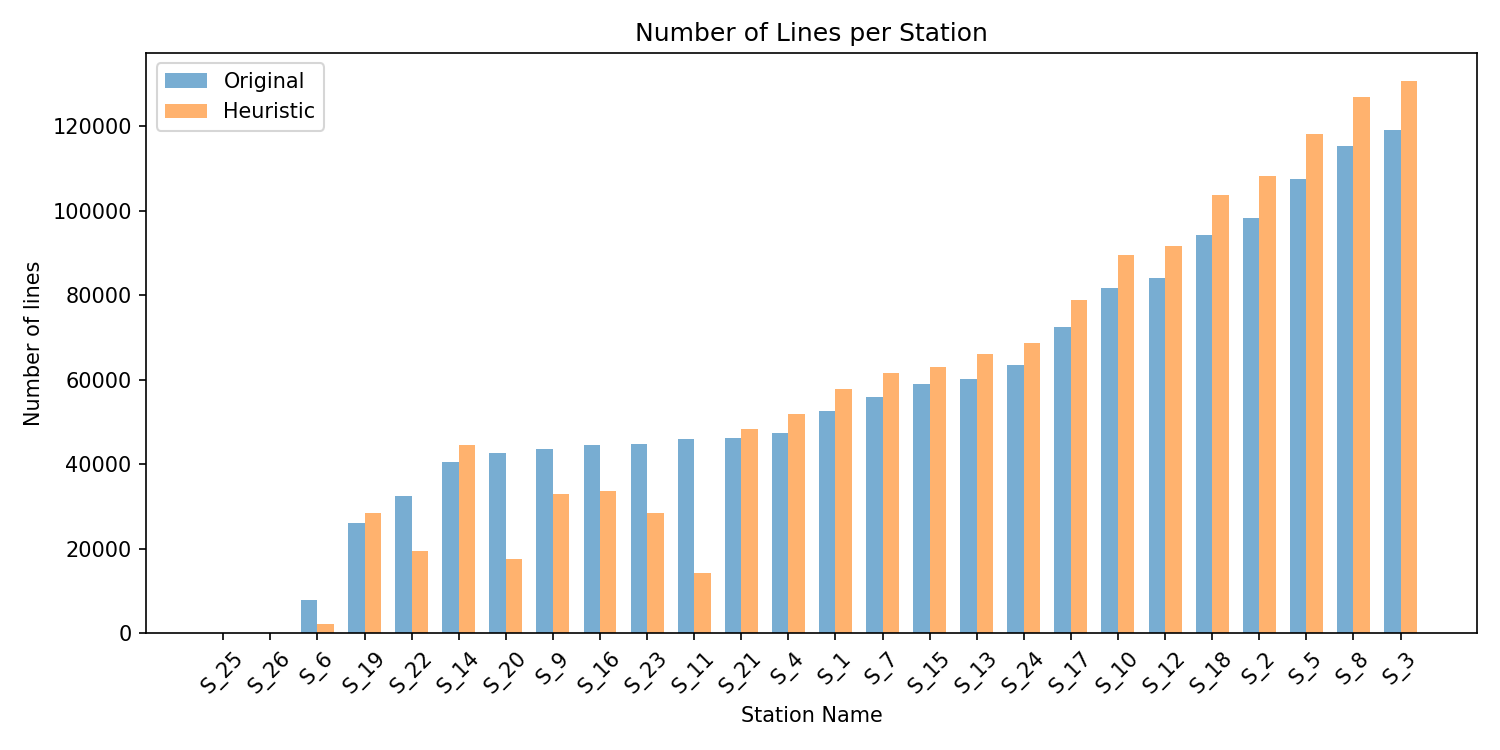
\includegraphics[width=\linewidth, height=4cm]{Images_CSLAP/r4_number_of_lines_per_station.png}
    \end{minipage}
    \hfill
    \begin{minipage}[b]{0.49\linewidth}
        \centering
        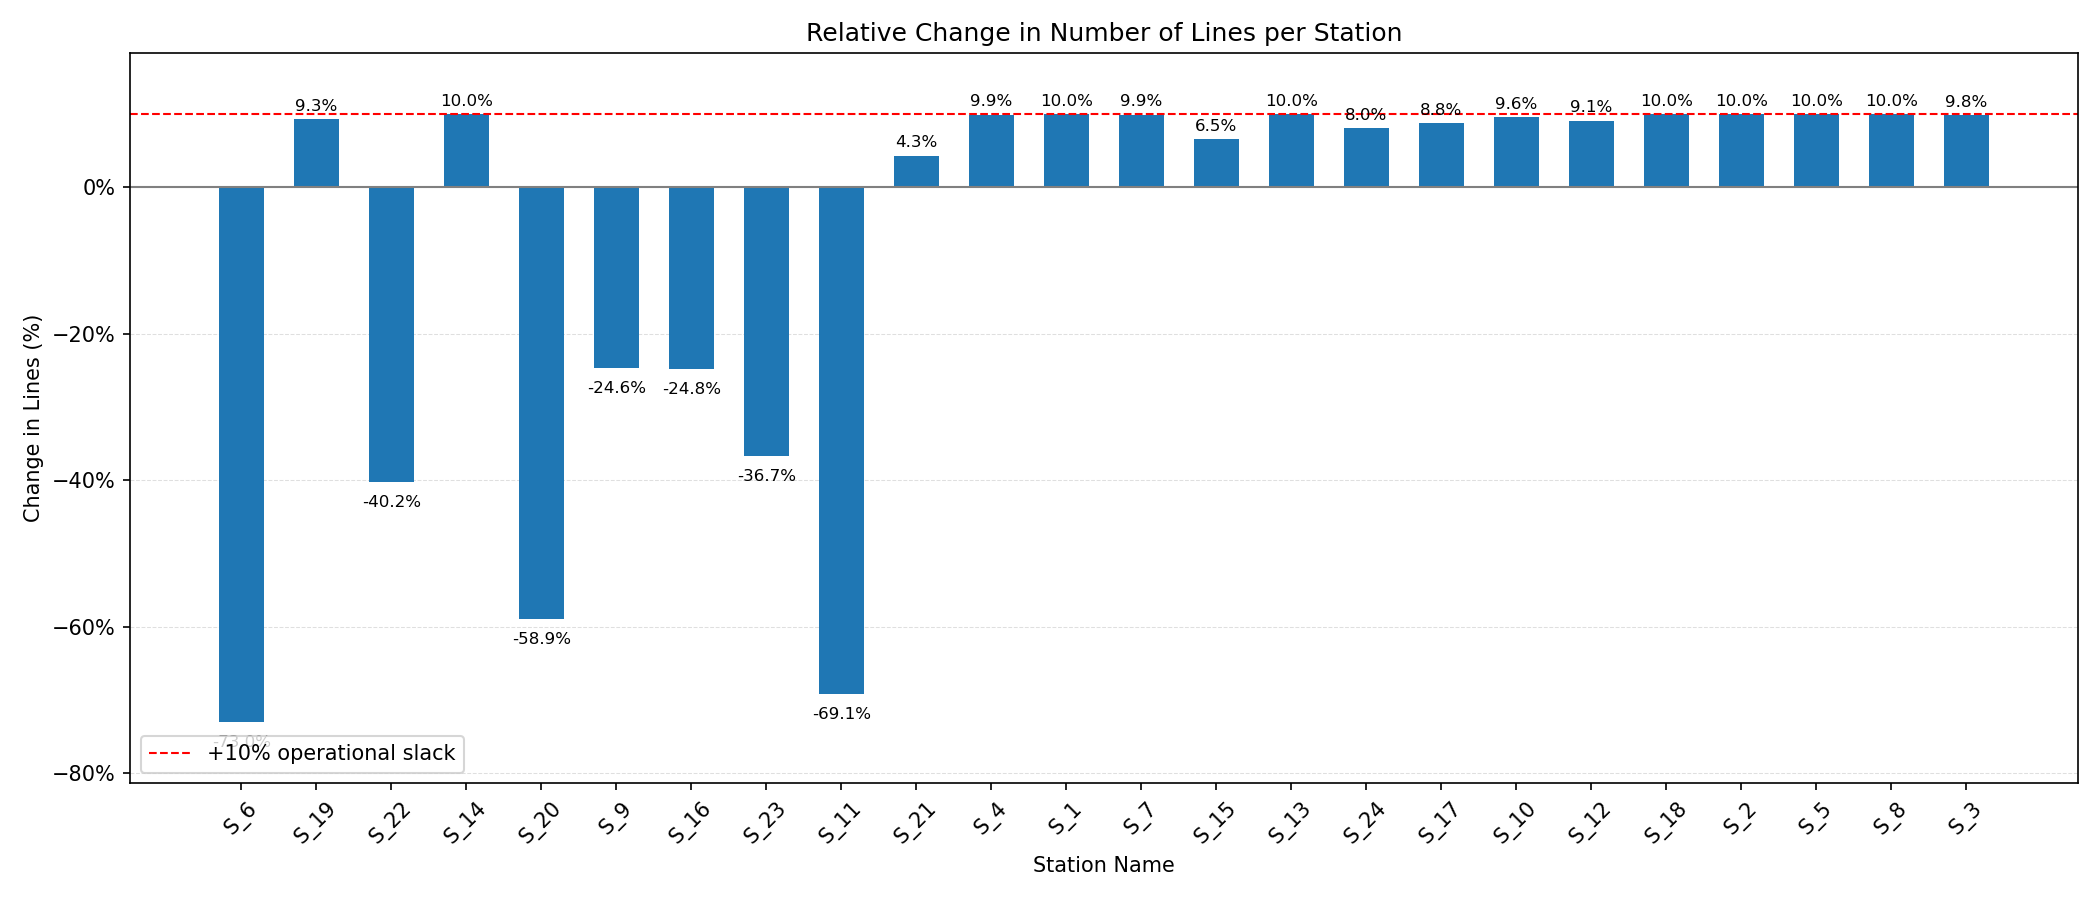
\includegraphics[width=\linewidth, height=4cm]{Images_CSLAP/r5_pct_change_lines_per_station.png}
    \end{minipage}
        \caption{Number of Lines per Station (left) and Relative Change Utilization Factor (right) resulting from the Heuristic assignment, compared against the Original Assignment.}
    \label{fig:comparison_lines_heuristic}
\end{figure}

\hyperref[fig:comparison_lines_heuristic]{Figure 3} illustrates the volatility of the heuristic assignment. While it successfully aggressively groups correlated items to reduce discrete stops, it mathematically disregards the strict workload boundaries. The right-hand graph displays massive relative percentage shifts in temporal workload, pushing several stations far beyond their engineered capacity limits (resulting in the WL violations noted in Table \ref{tab:industrial_21877sku}). Consequently, while the heuristic is a powerful tool for rapid, unconstrained clustering, its raw output may induce severe localized congestion if deployed without secondary balancing mechanisms.

\paragraph{\textbf{Exact Methods and the MILP Advantage}}
When scaling to the massive industrial instance of $21{,}874$ SKUs, the exact methods behave differently by formulation. To compare the set-partitioning column generation against the set-variable MILP on identical terms, we ran it on Company~A in its station-indexed form of \cref{sec:cg_master_general} under the MILP's exact inputs: the same per-station workload caps, the same solver-frequency workload basis, no lower bound on workload, and the identical full-evaluation used to score the MILP. The two methods therefore solve byte-for-byte the same constrained problem. As formalized in \cref{sec:cg_master_general}, each active station keeps its own convexity row in the master, and the single persistent pricing model serves all of them by swapping only the two station-dependent right-hand sides per call. Each station's workload cap is the MILP's own per-station cap, the engineered equilibrium of the site, so the run grants no capacity relief. Priced bundles are installed into the incumbent layout by an ejection-style recompletion that evicts the bundle's products, rebuilds the target station, and reinserts the displaced products by co-occurrence affinity, and the swap descent accepts moves lexicographically, feasibility strictly before visits. Over $106$ CG iterations the run generated $2{,}670$ columns with exact pricing at every iteration and used $35{,}940$ of the $36{,}000$ available seconds, improving the pruned-instance objective from the $680{,}270$-visit warm start to $627{,}523$. On the full evaluation the resulting layout scores $1{,}000{,}844$ visits, $9.09\%$ above the best feasible layout (set-variable MILP, $917{,}465$), and it improves the live legacy layout by $5.8\%$ ($61{,}663$ fewer visits). Under this fair setup the set-variable MILP retains the visit advantage at industrial scale, with column generation trailing it by $9.09\%$. Three strengths of the decomposition nevertheless stand. It is strictly feasible with the same violation profile as the MILP: neither method violates a solver-side cap, both exceed the raw current workload on ten stations under the full evaluation, and both remain within the site's $\pm 10\%$ operational tolerance, which is applied uniformly to every method at evaluation time; the column-generation layout's per-station deviations span $-3.8\%$ to $+5.8\%$, against $-5.9\%$ to $+9.6\%$ for the set-variable MILP. It disturbs the engineered utilization equilibrium the least among the optimizing methods, at $2.41$ standard deviation against $4.48$ for the set-variable MILP and $12.14$ for SA-C. And it completes and improves at this scale, where a conventional drive of the same per-station decomposition --- one pricing model per station, with an order-coverage variable for every order --- returns its warm start unchanged under the same ten-hour budget. The Farley pass ran to completion but stays uninformative at this scale, consistent with \cref{sec:cg_bound}. The remaining exact route to the deepest visit reduction is the set-variable MILP.

The MILP formulation powered by Hexaly's set-variable architecture successfully broke through the computational ceiling.

The structural trade-off between station-visit minimization and baseline workload preservation is illustrated by comparing the workload distributions of the set-variable MILP (\cref{fig:comparison_lines}) and Column Generation (\cref{fig:comparison_lines_cg}).

\begin{figure}[H]
    \centering
    \begin{minipage}[b]{0.49\linewidth}
        \centering
        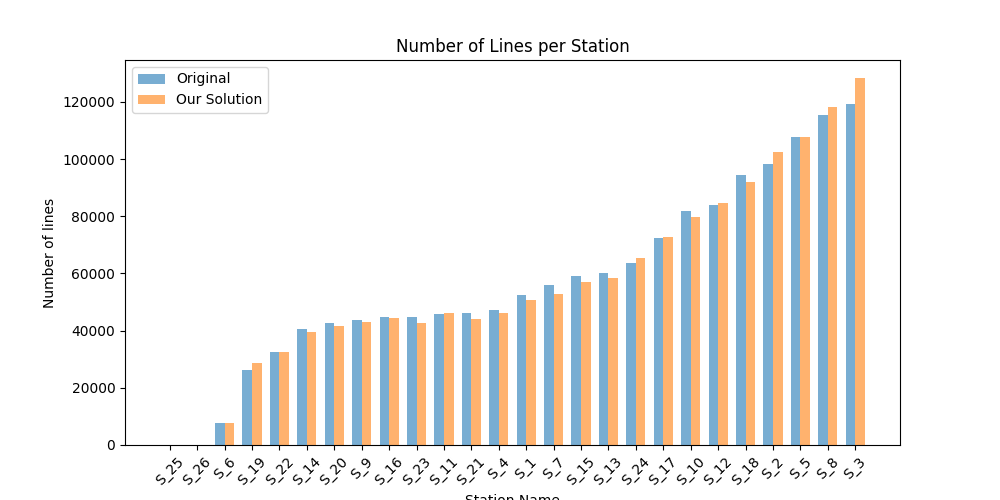
\includegraphics[width=\linewidth, height=4cm]{Images_CSLAP/Hexaly_number_of_lines_per_station.png}
    \end{minipage}
    \hfill
    \begin{minipage}[b]{0.49\linewidth}
        \centering
        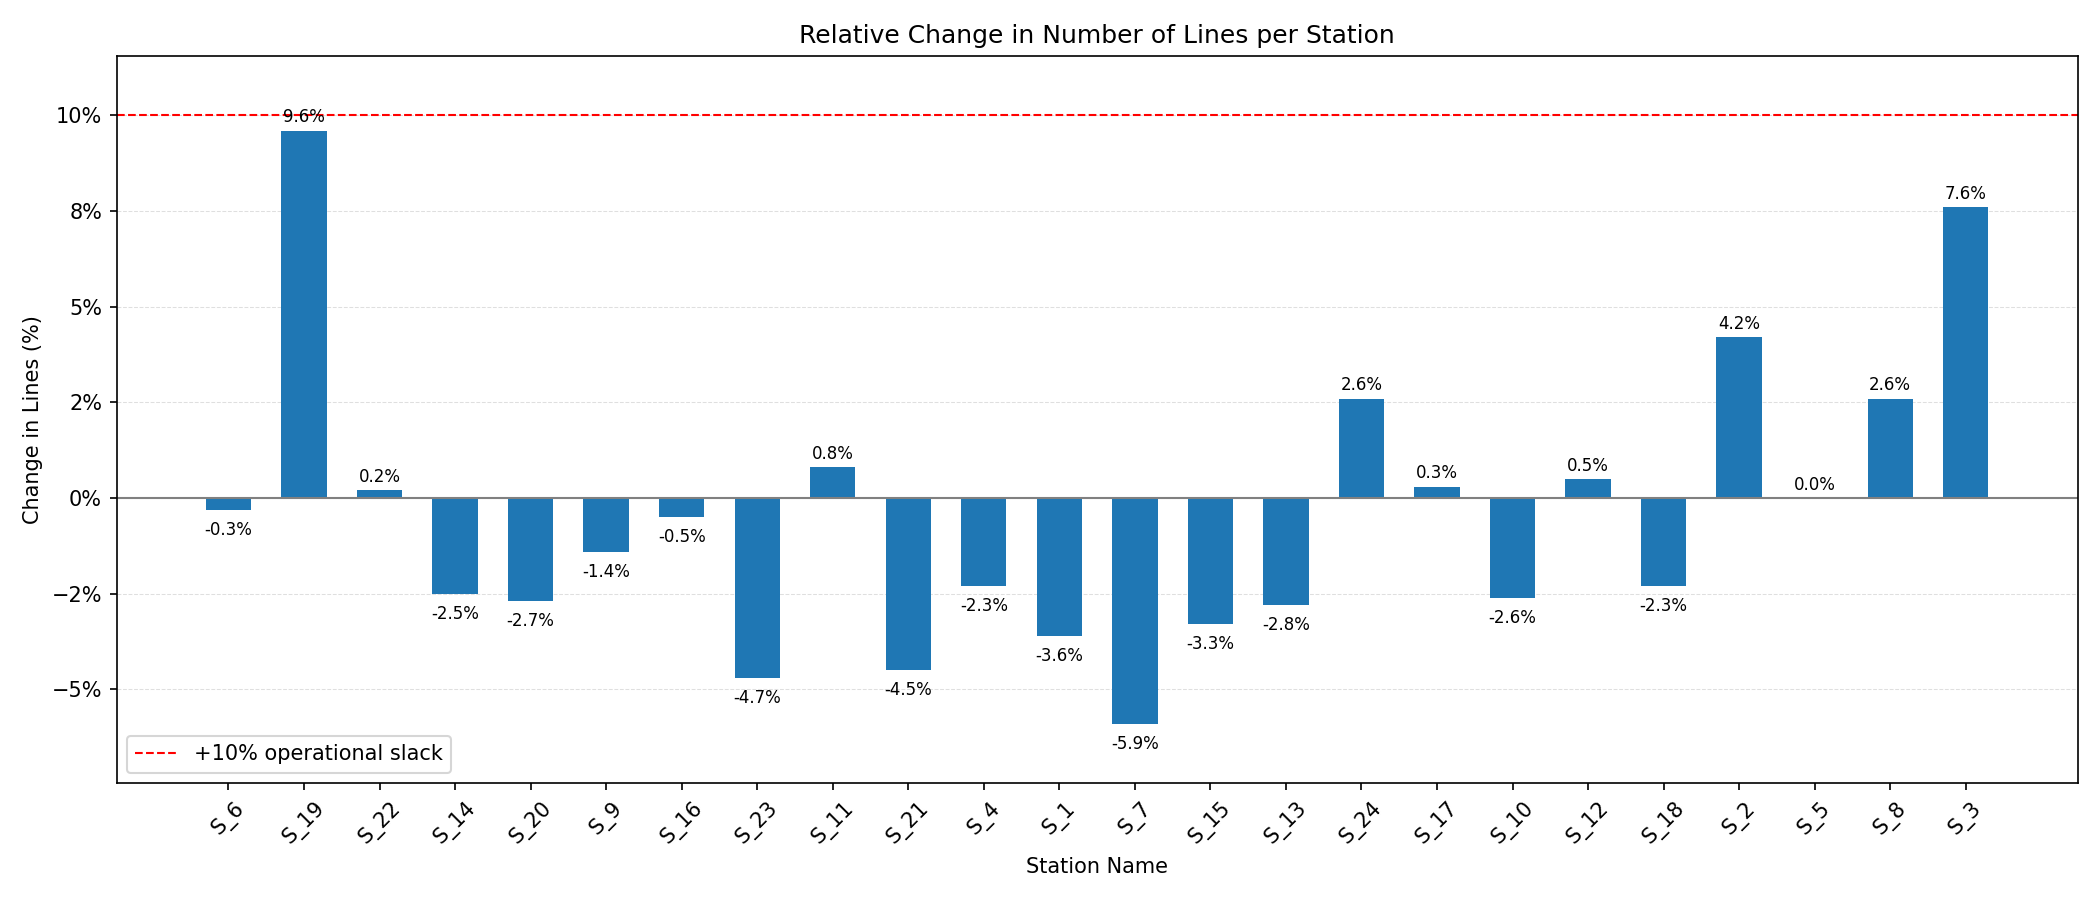
\includegraphics[width=\linewidth, height=4cm]{Images_CSLAP/Hexaly_pt_relative_change_number_of_lines_per_station.png}
    \end{minipage}
    \caption{Number of lines per station (left) and relative utilization change (right) for the set-variable MILP solution compared to the legacy assignment.}
    \label{fig:comparison_lines}
\end{figure}

\begin{figure}[H]
    \centering
    \begin{minipage}[b]{0.49\linewidth}
        \centering
        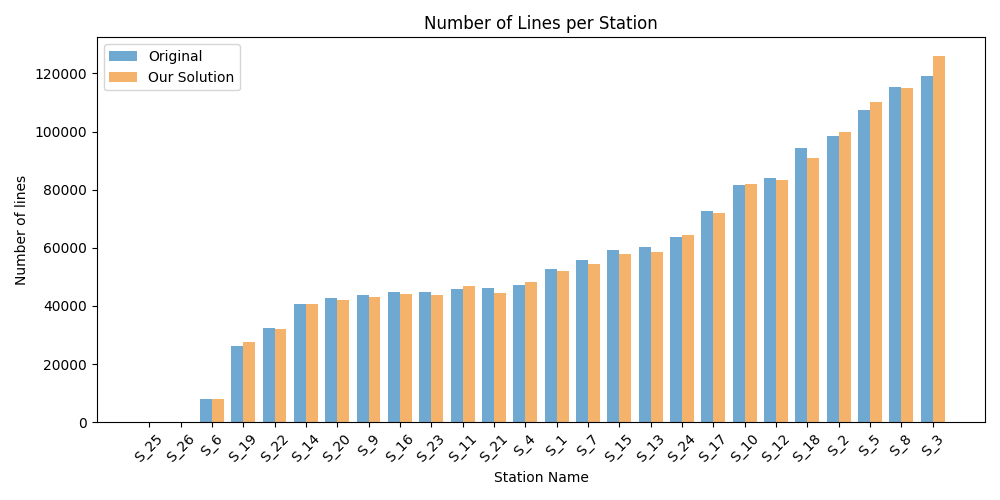
\includegraphics[width=\linewidth, height=4cm]{Images_CSLAP/cg_lines_per_station.png}
    \end{minipage}
    \hfill
    \begin{minipage}[b]{0.49\linewidth}
        \centering
        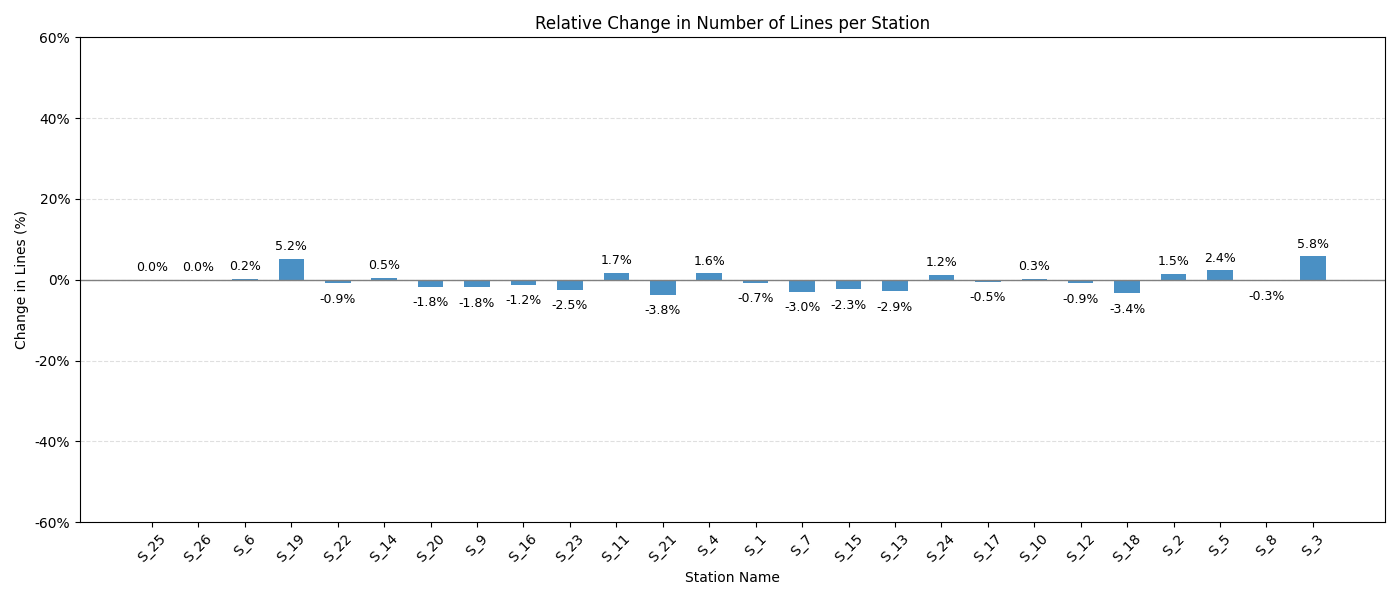
\includegraphics[width=\linewidth, height=4cm]{Images_CSLAP/cg_pct_change.png}
    \end{minipage}
    \caption{Number of lines per station (left) and relative utilization change (right) for the station-indexed Column Generation solution compared to the legacy assignment.}
    \label{fig:comparison_lines_cg}
\end{figure}

As shown in \cref{fig:comparison_lines}, the set-variable MILP solution achieves the deepest objective reduction ($917,465$ visits, a $13.7\%$ improvement over legacy) while maintaining strict operational feasibility. Its relative station workload shifts are bounded within $[-5.9\%, +9.6\%]$, yielding a standard deviation of $4.48\%$ across station utilization changes—well within the site's $\pm 10\%$ operational tolerance. The solver successfully rearranges the layout to eliminate stops without creating localized picking bottlenecks. This ability to break through the combinatorial wall stems from pairing the set-variable reformulation with Hexaly's hybrid local-search architecture, which effectively navigates the flat fitness landscape that stalls standard branch-and-bound \cite{blaisemodeling}.

Conversely, \cref{fig:comparison_lines_cg} confirms that the station-indexed Column Generation framework prioritizes workload stability above aggressive re-slotting. While achieving a $5.8\%$ visit reduction over legacy ($1,000,844$ visits), CG restricts relative workload deviations to a tight $[-3.8\%, +5.8\%]$ window, yielding the lowest utilization standard deviation among all optimizing methods ($2.41\%$). Graphically, the CG station loads track the engineered legacy baseline almost identically. This offers warehouse managers two distinct deployment profiles: the set-variable MILP when maximizing throughput velocity is paramount, and Column Generation when facility operations demand minimal perturbation to an established workload equilibrium.

\paragraph{\textbf{Real-World Labor Impacts: }}

\paragraph{\textbf{Real-World Labor Impacts: }}
The theoretical reduction in the objective function translates into massive logistical savings. Over the 66-day working quarter captured in our dataset, the original legacy layout required $1,062,507$ total station visits, averaging approximately $16,099$ daily stops. The optimized set-variable MILP layout reduces this total to $917,465$ visits. This yields a direct elimination of $145,042$ unnecessary mechanical stops and barcode scans per quarter. On a daily basis, this equates to roughly \textbf{2,198 fewer station visits per day}, representing a \textbf{13.7\%} structural drop in system congestion. This directly frees up roughly \textbf{nine full operating days} of picker and conveyor dwell time per quarter, allowing the facility to process identical order volumes with a significantly higher throughput velocity simply through intelligent re-slotting. We emphasise that these labor-day figures are linear extrapolations obtained by multiplying the eliminated visits by a fixed mechanical time-per-visit; they do not yet account for queueing or discrete-event dynamics, whose exact quantification we defer to the simulation study outlined in \cref{sec:conclusion}.

\paragraph{\textbf{Summary of Methodological Strengths: }}
The comparative analysis across the industrial dataset yields clear operational guidelines. The \textbf{Heuristic} approach is unmatched in computational speed and scalability, making it ideal for rapid, dynamic environments where strict workload balancing is less critical. The \textbf{set-variable MILP} stands as the superior framework for rigorous, scheduled re-slotting, providing the deepest reduction in station visits while guaranteeing strict adherence to physical and temporal capacity limits. Finally, \textbf{Column Generation} in its aggregated set-partitioning form matches the set-variable MILP on the homogeneous synthetic benchmark of \cref{sec:reliability_multiseed} while always respecting the workload cap, and in its station-indexed form (\cref{sec:cg_master_general}) it runs on Company~A as well. There it improves the live layout by $5.8\%$ and disturbs the utilization equilibrium the least among the optimizing methods at $2.41$ standard deviation while staying strictly feasible, though it trails the set-variable MILP on visits by $9.09\%$.

\subsection{Robustness validation via temporal hold-out}\label{sec:temporal_validation}

Having established the set-variable MILP formulation (solved via Hexaly) as the strongest framework for solution quality while strictly respecting workload boundaries, we now evaluate its operational resilience. To assess the robustness of the best-found assignments derived from limited historical data, we evaluate these layouts \emph{out of sample} by making optimized decisions on early weeks and testing them on later, unseen weeks.

This temporal hold-out mirrors realistic deployment (optimize once, then operate as demand evolves) and is consistent with robustness practices in storage assignment and warehouse optimization, where perfect information benchmarks (``oracle'' layouts) are contrasted with implementable policies \cite{lee2020cie,wang2020}. We performed two hold-out validation experiments on our 13-week dataset (3-month horizon) exclusively utilizing the set-variable MILP framework:

\begin{itemize}
  \item \textbf{Experiment 1:} The MILP makes decisions knowing only the first\,10 weeks of data, and the resulting layout is evaluated on the remaining 3 weeks.  
  \item \textbf{Experiment 2:} The MILP makes decisions knowing only the first\,8 weeks of data, and the resulting layout is evaluated solely on the final 5 weeks.
\end{itemize}

These out-of-sample solutions are benchmarked against the original placement and against the “oracle” layout obtained when the MILP is optimized directly on the hold-out weeks with perfect future knowledge.

\begin{table}[H]
\centering
\small
\renewcommand{\arraystretch}{1.1}
\setlength{\tabcolsep}{6pt}
\begin{tabular}{@{}llcc@{}}
\toprule
\textbf{Validation} & \textbf{Layout (Training Period)} & \textbf{Total Visits} & \textbf{Avg. Visits} \\
\midrule
\multirow{3}{*}{Last 3 weeks} & Baseline (Original placement) & 265,876 & 4.052 \\
& MILP (optimised on first 10 weeks) & 248,358 & 3.785 \\
& MILP Oracle (optimised on last 3 weeks) & 233,728 & 3.562 \\
\midrule
\multirow{3}{*}{Last 5 weeks} & Baseline (Original placement) & 423,593 & 3.926 \\
& MILP (optimised on first 8 weeks) & 392,318 & 3.636 \\
& MILP Oracle (optimised on last 5 weeks) & 380,356 & 3.525 \\
\bottomrule
\end{tabular}
\caption{Station-visit performance evaluated on distinct hold-out validation periods.}
\label{tab:temporal_validation}
\end{table}

\paragraph{\textbf{Discussion}}
The results of the validation experiments demonstrate the practical robustness of decisions derived from limited historical data: \\
\textbf{Experiment 1:} Using only the first 10 weeks cuts station visits by 6.6\% versus the baseline, while the oracle, optimized directly on the test weeks, achieves 12.1\%. This gap ($\approx$5\%) shows that some short-term seasonal effects are missed, yet the vast majority of the structural affinity benefit is captured. \\
\textbf{Experiment 2:} With eight weeks of history, the MILP reduces visits by 7.4\%; the oracle gains 10.2\%. Again, historical correlations yield a strong but not exhaustive improvement. 

Thus, for this \textit{specific warehouse}, the recent past provides guidance that is \emph{good enough for meaningful savings}, although not completely predictive. However, we acknowledge such stability might vary in different operational contexts. Hence, future work should explore incorporating predictive models or stochastic scenario planning to further manage demand uncertainties.

\subsection{Practical Extension: Limited Product Reassignment}
\label{sec:limited_reassignment}

While the set-variable MILP (solved via Hexaly) yields the lowest station-visit count we obtain, fully redesigning an active 21,874-SKU warehouse layout is often operationally disruptive. Moving every product to its newly assigned position requires extended downtime and significant labor, risking delays in fulfillment.

To provide a cost-effective, continuous-improvement strategy, we introduce a practical extension to our base LP model that restricts the total number of products allowed to be relocated. By capping the reassignment at a maximum boundary $k$, managers can match the re-slotting effort to their available workforce while capturing the most critical throughput benefits.

\subsubsection{Mathematical Formulation with Limited Reassignment}
To model this within our MILP framework, we build upon the decision variables established in \cref{sec:LP_Approach}. We define a constant parameter $s'(p) \in S$, which represents the \emph{original} (legacy) station assignment of product $p$.

Recall that our binary decision variable $x_{ps} \in \{0,1\}$ equals 1 if product $p$ is assigned to station $s$ in the newly optimized layout. Therefore, the specific variable $x_{p, s'(p)}$ equals 1 if and only if product $p$ remains in its original legacy station. We append a single global constraint to the MILP formulation:
\begin{equation}
\sum_{p \in P} x_{p,s'(p)} \ge |P| - k
\label{constraint:reassignment}
\end{equation}
Constraint~\eqref{constraint:reassignment} enforces that the total number of products staying in their original locations must be at least $|P| - k$. Equivalently, this ensures the total number of relocated products across the entire warehouse is strictly bounded to at most $k$.

\subsubsection{Quantitative Analysis: the Effort--Benefit Trade-off}
Rather than fixing a single relocation budget, we characterise how the achievable benefit scales with $k$. We re-solved the industrial instance under a sweep of caps, $k \in \{250, 500, 1{,}000, 2{,}000, 5{,}000\}$, each under a uniform one-hour solver budget, and contrast the result against both the legacy layout ($k=0$) and the full re-optimization anchor (the $917{,}465$-visit solution of \cref{tab:industrial_21877sku}, which required a ten-hour budget). \Cref{tab:restricted_MILP} and \cref{fig:ksweep} report the trade-off.

\begin{table}[H]
  \centering
  \small\setlength{\tabcolsep}{5pt}
  \begin{threeparttable}
  \begin{tabularx}{\linewidth}{@{}l*5{>{\centering\arraybackslash}X}@{}}
    \toprule
    \textbf{Relocation cap} & \textbf{\% catalog} & \textbf{Total visits} & \textbf{Reduction} & \textbf{\% of full benefit} & \textbf{WL-viol.\ stations} \\
    \midrule
    Legacy ($k=0$)        & 0\%     & 1,062,507 & --       & --      & 0 \\
    $k=250$               & 1.1\%   & 1,061,302 & 1,205    & 0.8\%   & 0 \\
    $k=500$               & 2.3\%   & 1,060,120 & 2,387    & 1.6\%   & 0 \\
    $k=1{,}000$           & 4.6\%   & 1,056,412 & 6,095    & 4.2\%   & 0 \\
    $k=2{,}000$           & 9.1\%   & 1,049,730 & 12,777   & 8.8\%   & 0 \\
    $k=5{,}000$           & 22.9\%  & 1,034,735 & 27,772   & 19.2\%  & 0 \\
    \midrule
    Full re-opt.\tnote{a} & --      & 917,465   & 145,042  & 100\%   & 0 \\
    \bottomrule
  \end{tabularx}
  \begin{tablenotes}\footnotesize
    \item[a] Unrestricted set-variable MILP from \cref{tab:industrial_21877sku} (ten-hour budget); shown as the asymptotic reference.
  \end{tablenotes}
  \end{threeparttable}
    \caption{Limited-reassignment trade-off on the industrial dataset: visit reduction as a function of the relocation cap $k$. ``\% of full benefit'' is the reduction relative to the $145{,}042$-visit full re-optimization. ``WL-viol.\ stations'' counts stations whose realised workload exceeds the cap.}
    \label{tab:restricted_MILP}
\end{table}

\begin{figure}[H]
    \centering
    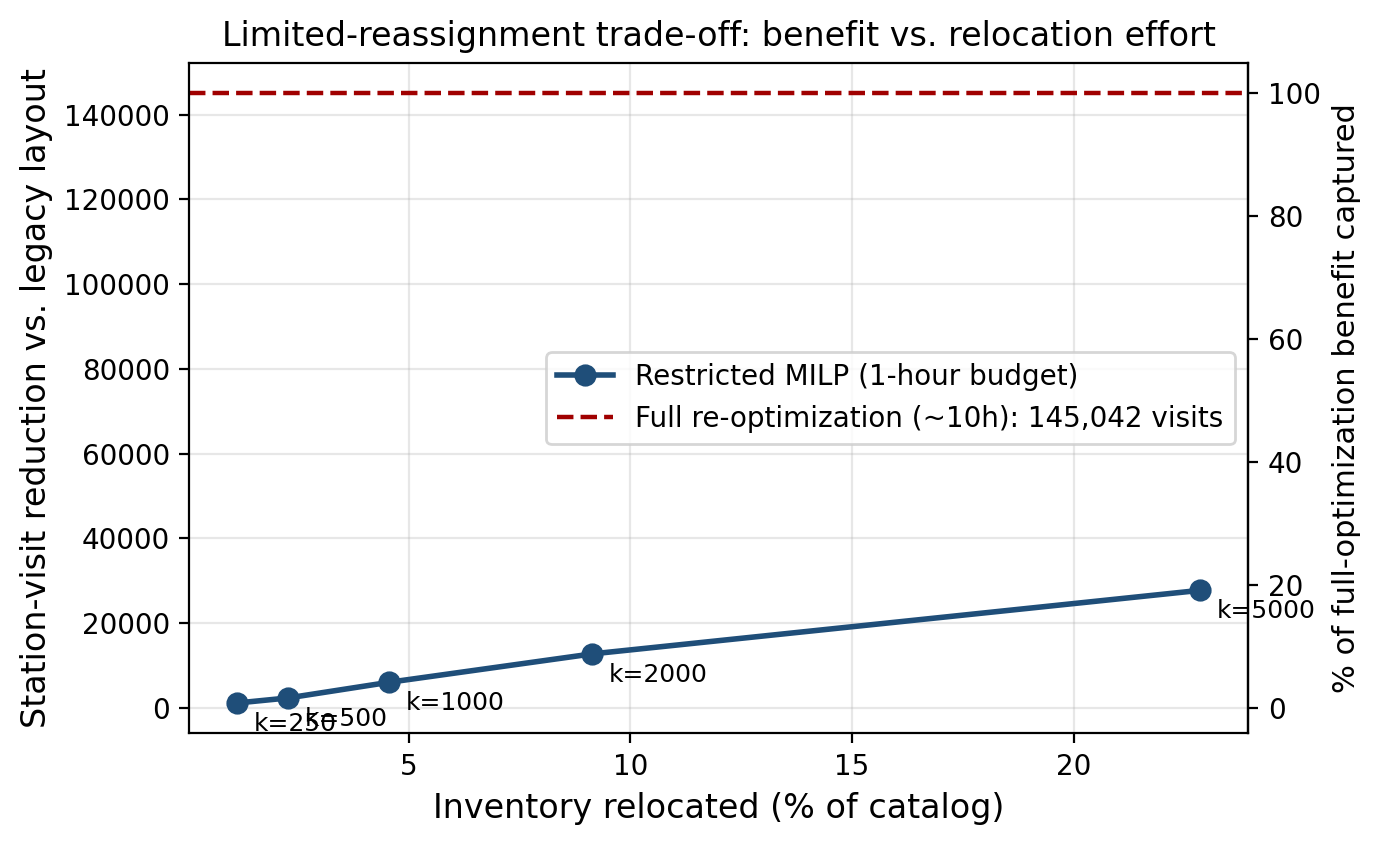
\includegraphics[width=0.78\linewidth]{Images_CSLAP/reassignment_ksweep_curve.png}
    \caption{Station-visit reduction versus the fraction of the catalog relocated. The dashed line marks the full re-optimization benefit ($145{,}042$ visits). The benefit accrues gradually with relocation effort rather than concentrating in a small fraction of moves.}
    \label{fig:ksweep}
\end{figure}

Two findings emerge. First, the benefit of restricted re-slotting accrues roughly in step with the relocation effort: relocating $2.3\%$ of the catalog captures $1.6\%$ of the full reduction, and relocating $22.9\%$ captures $19.2\%$. No small subset of moves captures a disproportionate share of the gain, so most of the improvement in the full solution still comes from a large-scale rearrangement that a tightly bounded budget cannot reproduce. The curve therefore quantifies what a manager forgoes by limiting disruption, and lets the relocation budget $k$ be chosen to match available labor against a known marginal benefit.

Second, every restricted layout is operationally feasible. At each cap the solver keeps every station within both its storage capacity and its workload budget, and it barely disturbs the engineered balance of the site: the busiest station load and the spread of utilisation across stations stay essentially at their legacy values. The whole trade-off curve is therefore deployable as it stands, and a manager can adopt any point on it without a separate workload-repair pass or a longer overnight solve. This is a direct consequence of reserving each station's residual time budget for the frozen low-frequency products before the restricted search begins, which prevents the relocated items from crowding a zone.




\section{Conclusion}
\label{sec:conclusion}

In this study, we proposed a fundamental paradigm shift for the Correlated Storage Location Assignment Problem (CSLAP) in automated, conveyor-driven warehouses. Moving away from traditional travel-distance metrics, we formulated a rigorously constrained mathematical framework explicitly designed to minimize discrete station visits per order while enforcing strict workload synchronization across heterogeneous picking zones. Through comprehensive benchmarking on synthetic datasets and a massive 21,874-SKU industrial instance, we established a critical computational insight: framing CSLAP to minimize discrete station stops creates an exceptionally flat fitness landscape. Consequently, probabilistic searches (GA, SA-C) and classical binary branch-and-bound stall in this environment. We found empirically that high solution quality together with operational feasibility at an industrial scale is best achieved by pairing a subset-based set-variable reformulation with a hybrid local-search engine and rigorous workload capacity constraints. By extending this model with a limited-reassignment boundary, we showed how managers can trade re-slotting effort against throughput gain through a single relocation budget, rendering targeted mathematical re-slotting practically viable for active, large-scale facilities.

\subsection*{Managerial Implications and Practical Applicability}

Beyond the theoretical advancements, this research provides an actionable, highly scalable toolkit for warehouse operations leaders. By bridging the gap between exact mathematical modeling and operational realities, we distill four primary directives for industry practice:

\begin{itemize}
    \item \textbf{Adopt station-visits as a primary slotting KPI.} In conveyor and zone-routing systems, discrete station stops directly generate mechanical queuing and handling delays. Tracking ``stops per order'' reveals congestion hot spots that traditional distance-only metrics obscure.
    \item \textbf{Match the algorithmic tool to the operational urgency.} Our framework empowers managers to tailor their optimization strategy. For rapid, daily dynamic clustering where workload balance is flexible, our parameter-free heuristic executes in seconds. For scheduled, quarterly facility overhauls, the set-variable MILP solved with a hybrid local-search engine produces the highest-quality layouts we obtain. In our industrial case study, this set-variable hybrid approach delivered a 13.7\% structural reduction in the objective function, eliminating approximately 2,198 mechanical stops per day and freeing roughly nine full operating days of conveyor dwell time per quarter (a linear extrapolation under a fixed time-per-visit assumption).
    \item \textbf{Drive continuous improvement via restricted re-slotting.} Recognizing the prohibitive cost and disruption of massive layout overhauls, operations leaders should utilize our limited-reassignment MILP extension. We characterise how the achievable visit reduction grows with the relocation budget $k$, enabling surgical throughput upgrades matched to available labor without facility downtime.
    \item \textbf{Recalibrate using a rolling historical window.} Our temporal hold-out analysis proves that layouts optimized on a recent 8-to-10-week window of order data generalize robustly to the subsequent month. Implementing this rolling optimization cycle maintains peak performance while limiting continuous engineering effort.
\end{itemize}




\section {Future Research Directions}\label{sec:future}
While this research establishes a robust foundation for station-visit minimization, several avenues remain for future exploration. 

First, several algorithmic extensions would strengthen the set-partitioning column generation. Dual stabilization, for instance the du~Merle box or a Wentges center, would tighten the Farley certificate that is currently loose at scale and turn the matheuristic reading into certified gaps. A branch-and-price layer on top of the price-and-complete dive would then let the certified bound and the primal search close the remaining gap. On the industrial side the station-indexed run of \cref{sec:numerical_results} already improves the live layout feasibly, but it trails the set-variable MILP on visits by $9.09\%$; closing that gap, either through a longer optimization horizon or by hybridizing the swap descent with the set-variable engine, is the remaining industrial lever.

Second, operational realism can be further enhanced by incorporating heterogeneous product geometries and 3D bin-packing constraints within the station capacities, moving beyond simple SKU counting. 

Finally, while our mathematical models implicitly reduce expected queuing via workload balancing, integrating these layouts into high-fidelity discrete-event simulations will allow for the exact quantification of micro-level queue dynamics and throughput gains. Expanding the models to accommodate stochastic demand patterns and real-time routing logic will ultimately secure resilient, high-performance warehouse operations in increasingly volatile e-commerce supply chains.



% ---------------------------------------------------------------
% DECLARATIONS (BLINDED FOR PEER REVIEW)
% ---------------------------------------------------------------

% ---> PLACE THE DATA AVAILABILITY STATEMENT HERE <---

\section*{Data availability statement}
The synthetic data sets, generation scripts, and all benchmarking and limited-reassignment experiment code used in this study are openly available in an anonymized repository at \url{https://anonymous.4open.science/r/Anonymized_Export_CSLAP-1876/} (the de-anonymized permanent repository link will be provided on acceptance). The real-world industrial data set used in \cref{sec:numerical_results} (Company A) is not publicly available due to strict commercial confidentiality restrictions.

% \section*{Funding}
% This research was carried out with the support of the Association Nationale de la Recherche et de la Technologie (ANRT), Savoye, and the University of Technology of Compiègne.

% \section*{Acknowledgments}
% The authors thank the operational teams at Company A for providing the industrial dataset and their insights into the automated picking processes. 

% \section*{Declaration of Generative AI in scientific writing}
% During the preparation of this work, the authors used Google Gemini 3 to assist with language refinement. After using this tool, the authors rigorously reviewed and edited the content as needed and take full responsibility for the content, integrity, and accuracy of the publication.

% \section*{CRediT authorship contribution statement}
% \textbf{Ermal Belul:} Conceptualization, Methodology, Software, Data curation, Investigation, Formal analysis, Visualization, Writing   original draft, Writing   review \& editing. 
% \textbf{Marwane Bouznif:} Conceptualization, Supervision, Validation, Writing   review \& editing.  
% \textbf{Dritan Nace:} Conceptualization, Supervision, Validation, Writing   review \& editing.  
% \textbf{Antoine Jouglet:} Conceptualization, Supervision, Validation, Writing   review \& editing.

\section*{Disclosure statement}
The authors report there are no competing interests to declare.


% % --------------------- Declarations & statements ------------
% \section*{Credit authorship contribution statement}

% \textbf{Ermal Belul}: Conceptualization, Methodology, Software, Data curation, Investigation, Formal analysis, Visualization, Project administration, Writing – original draft, Writing – review \& editing. 
% \textbf{Marwane Bouznif}: Conceptualization, Supervision, Validation, Writing – review \& editing.  
% \textbf{Dritan Nace}: Conceptualization, Supervision, Validation, Writing – review \& editing.  
% \textbf{Antoine Jouglet}: Conceptualization, Supervision, Validation, Writing – review \& editing.

% \section*{Acknowledgments}
% This research was carried out with the support of the Association Nationale de la Recherche et de la Technologie (ANRT), Savoye, and the University of Technology of Compiègne.

% \section*{Declaration of competing interest}
% The authors declare that they have no known competing financial interests or personal relationships that could have appeared to influence the work reported in this paper.

\bibliographystyle{cas-model2-names}

\begin{thebibliography}{00}

% \bibitem[(Ansari and Smith, 2020)]{ansari2020}
% Ansari, M., Smith, J.S., 2020. Gravity clustering: A correlated storage location assignment problem approach. In: Proceedings of the 2020 Winter Simulation Conference, 1288-1299.

\bibitem[(Azadeh et al., 2019)]{azadeh2019}
Azadeh, K., De Koster, R., Roy, D., 2019. Robotized and Automated Warehouse Systems: Review and recent developments. \textit{Transportation Science}, 53(4), 917-945.

% \bibitem[(Belul et al., 2025)]{ErmalBelul2025}
% Belul, E., Bouznif, M., Nace, D., Jouglet, A., 2025. Optimizing Automated Warehouse Operations: A Novel Approach to the Correlated Storage Location Assignment Problem (CSLAP), 20th Annual System of Systems Engineering Conference (SoSE), Tirana, Albania, 2025

\bibitem[(Blaise, Hexaly)]{blaisemodeling}
Blaise, L., n.d. Modeling scheduling problems with Hexaly. Hexaly, 251 Boulevard Pereire, 75017 Paris, France.

\bibitem[(Boysen et al., 2023)]{boysen2023}
Boysen, N., Schwerdfeger, S., Stephan, K., 2023. A review of synchronization problems in parts-to-picker warehouses. \textit{European Journal of Operational Research}, 307(3), 1374-1390.

\bibitem[(Kim and Smith 2012)]{kim2012}
Kim, Byung S., Smith, Jeffrey S.,2012
Slotting methodology using correlated improvement for a zone-based carton picking distribution system
\textit{Computers \& Industrial Engineering 62(1), 286-295}

% \bibitem[(Caprara et al.,2000)]{caprara2000algorithms}
% Caprara, A., Fischetti, M., Toth, P., 2000. Algorithms for the set covering problem. \textit{Annals of Operations Research 98(1-4), 353-371.}

\bibitem[(Chabot et al.,2024)]{chabot2024reassignment}
Chabot, T., et al., 2024. Reassignment problem. In: Warehousing and Material Handling Systems for the Digital Industry, p.~137.

\bibitem[Chuang et al. (2016)]{chuang2016}
Chuang, Y. et al. 2016. A robust heuristic method on the clustering-assignment problem model
\textit{Computers \& Industrial Engineering}, 98, 63-67.


\bibitem[(Desrochers and Soumis, 1989)]{desrochers1989column}
Desrochers, M., Soumis, F., 1989. A column generation approach to the urban transit crew scheduling problem. \textit{Transportation Science} 23(1), 1-13.

% \bibitem[(Egas and Masel, 2010)]{Egas2010-zb}
% Egas, C., Masel, D., 2010. Determining warehouse storage location assignments using clustering analysis. In: Proceedings of the 11th IMHRC, Milwaukee, WI.

\bibitem[(Farley, 1990)]{farley1990note}
Farley, A.A., 1990. A note on bounding a class of linear programming problems, including cutting stock problems. \textit{Operations Research} 38(5), 922-923.

\bibitem[(Garey and Johnson, 1979)]{garey1979computers}
Garey, M.R., Johnson, D.S., 1979. \textit{Computers and Intractability: A Guide to the Theory of NP-Completeness}. W. H. Freeman.

\bibitem[(Islam and Uddin, 2023)]{islam2023}
Islam, M.S., Uddin, M.K., 2023. Correlated storage assignment approach in warehouses: A systematic literature review. Journal of Industrial Engineering and Management 16(2), 294--318.

\bibitem[(Kim and Hong, 2020)]{kim2020}
Kim, T., Hong, S., 2020. Two Picker Cooperation Strategies for Zone
Picking Systems With PTL Technology. \textit{IEEE Xplore}, https://ieeexplore.ieee.org/document/9106329

\bibitem[Lee et al.(2020)]{lee2020cie}
Lee, I.G., Chung, S.H., Yoon, S.W. (2020).
Two-stage storage assignment to minimize travel time and congestion for warehouse order picking operations.
\textit{Computers \& Industrial Engineering}, 139, 106129.
%https://doi.org/10.1016/j.cie.2019.106129

% \bibitem[Liu and Poh(2023)]{liu2023scattered}
% Liu, M., Poh, K.L. (2023).
% E-commerce warehousing: An efficient scattered storage assignment algorithm with bulky locations.
% \textit{Computers \& Industrial Engineering}, 181, 109236.
%https://doi.org/10.1016/j.cie.2023.109236

\bibitem[(L{\"u}bbecke and Desrosiers , 2005)]{lubbecke2005selected}
L{\"u}bbecke, M.E., Desrosiers, J., 2005. Selected topics in column generation.
\textit{Operations Research} 53(6), 1007-1023. 
%https://doi.org/10.1287/opre.1050.0234

\bibitem[(Mirzaei et al., 2022)]{mirzaei2021}
Mirzaei, M., Zaerpour, N., De Koster, R., 2022. How to benefit from order data: correlated dispersed storage assignment in robotic warehouses. \textit{International Journal of Production Research}, 60(2), 549--568.

\bibitem[(Muter and Oncan, 2022)]{muter2022}
Muter, I., Oncan, T., 2022. Order batching and picker scheduling in warehouse order picking. \textit{IISE Transactions}, 54(5), 435--447.


\bibitem[(Pan et al., 2015)]{pan2015}
Pan, J.C.H., Shih, P.H., Wu, M.H., 2015. Order batching in a pick-and-pass warehousing system with group genetic algorithm. \textit{Omega}, 57, 238-248.

% \bibitem[(Pang and Chan, 2016)]{pang2016}
% Pang, K.-W., Chan, H.-L., 2016. Data-mining-based algorithm for storage location assignment in a randomised warehouse. International Journal of Production Research 55(14), 4035-4052.

\bibitem[(Tarczyński, 2023)]{tarczynski2023}
Tarczyński, G., 2023. Linear programming models for optimal workload
and batching in pick-and-pass warehousing systems. \textit{Operations Research and Decisions}, DOI:10.37190/ord230309
Authors:

\bibitem[(Vanderbeck, 2000)]{vanderbeck2000dw}
Vanderbeck, F., 2000. On Dantzig-Wolfe decomposition in integer programming and ways to perform branching in a branch-and-price algorithm. \textit{Operations Research} 48(1), 111-128.

\bibitem[(Teun van Gils et al., 2018)]{vanGils2018}
van Gils, T., Ramaekers, K., Caris, A., de Koster, R., 2018. Designing efficient order picking systems by combining planning problems: State-of-the-art classification and review. \textit{European Journal of Operational Research}, 267(1), 1-15.

% \bibitem[(Trindade et al., 2022)]{trindade2022}
% Trindade, M.A.M., Sousa, P.S.A., Moreira, M.R.A., 2022. Ramping up a heuristic procedure for the storage location assignment problem with precedence constraints. Flexible Services and Manufacturing Journal 34(3), 646-669.

\bibitem[(Wang et al., 2020)]{wang2020}
Wang, M., Zhang, R.-Q., Fan, K., 2020. Improving order-picking operation through efficient storage location assignment: A new approach. \textit{Computers \& Industrial Engineering}, 139, 106186.
%https://doi.org/10.1016/j.cie.2019.106186

\bibitem[(West et al., 2001)]{west2001introduction}
West, D.B., et al., 2001. \textit{Introduction to Graph Theory} (Vol. 2). Prentice Hall.

\bibitem[(Xiao and Zheng, 2010)]{xiao2010correlated}
Xiao, J., Zheng, L., 2010. A correlated storage location assignment problem in a single-block multi-aisle warehouse considering bill-of-material information. International Journal of Production Research 48(5), 1321--1338.

\bibitem[(Xie and Otten, 2024)]{xie2024combi}
Xie, L., Otten, S., 2024. Introducing combi-stations in robotic mobile fulfilment systems: A queueing-theory-based efficiency analysis. In: International Conference on Computational Logistics. Springer.

\bibitem[(Xie et al., 2021)]{xie2021}
Xie, L., Thieme, N., Krenzler, R., Li, H., 2021. Introducing split orders and optimizing operational policies in robotic mobile fulfillment systems. \textit{European Journal of Operational Research}, 288(1), 80--97.

\bibitem[Zhang et al.(2019)]{zhang2019cie}
Zhang, R.-Q., Wang, M., Pan, X. (2019).
New model of the storage location assignment problem considering demand correlation pattern.
\textit{Computers \& Industrial Engineering}, 129, 210-219.
%https://doi.org/10.1016/j.cie.2019.01.027


% \bibitem[Zhang et al.(2023)]{zhang2023rmfs}
% Zhang, J., Zhang, N., Tian, L., Zhou, Z., Wang, P. (2023).
% Robots’ picking efficiency and pickers’ energy expenditure: The item storage assignment policy in robotic mobile fulfillment system.
% \textit{Computers \& Industrial Engineering}, 176, 108918.
%https://doi.org/10.1016/j.cie.2022.108918


\bibitem[(Zhen et al., 2025)]{zhen2025}
Zhen, L., Tan, Z., de Koster, R., He, X., Wang, S., Wang, H., 2025. Optimizing Warehouse Operations with Autonomous Mobile Robots. \textit{Transportation Science}, forthcoming.

\bibitem[(Zhu et al., 2021)]{zhu2021}
Zhu, S., Hu, X., Huang, K., Yuan, Y., 2021. Optimization of product category allocation in multiple warehouses to minimize splitting of online supermarket customer orders. \textit{European Journal of Operational Research}, 291(2), 642-658.

\end{thebibliography}
\newpage

\appendix
\section{Detailed Heuristic Pseudocode}
\label{sec:appendix_heuristic}

The following algorithm details the exact procedural logic of the Greedy Product Clustering heuristic summarized in \cref{sec:methodology}.

\noindent The core algorithm of our heuristic is:

\begin{algorithm}[H]
\caption{Algorithm 1: Greedy Product Clustering and Station Assignment (CSLAP)}
\label{alg:greedy-cslap}
\begin{algorithmic}[1]

\Statex \textbf{Step 1: Preprocessing and Pair Generation.}
\begin{enumerate}[label=(\alph*)]
\item Define $P^*=\{\,p\in P:\mathrm{freq}(p)\ge \mathrm{MIN\_FREQ\_PREPROC}\,\}$.
\item For each multi-item order $o\in O$, generate all unordered pairs $(p_i,p_j)$ with $p_i,p_j\in P^*$ and $i<j$.
\item Compute the co-occurrence count : \(\mathrm{count_{ij}} = \big|\{\,o \in O : \{p_i,p_j\} \subset o | i < j \}\big|, \)
and keep only pairs with $\mathrm{count}_{ij}\ge \mathrm{MIN\_FREQ}$.
\item For each kept pair, compute $\eta_{ij}=\mathrm{count}_{ij}/\mathrm{count}_i$ and retain those with $\eta_{ij}\ge \mathrm{RATIO\_TO\_KEEP}$.
\item Sort remaining pairs in descending $\mathrm{count}_{ij}$ (ties arbitrary).
\end{enumerate}
\medskip
\textbf{Step 2: Community Formation.}
\begin{enumerate}[label=(\alph*)]
\item Initialize the set of communities $\mathcal{C}\leftarrow\varnothing$; mark all products as “unassigned”.
\item While there are candidate pairs left:
  \begin{enumerate}[label*=\arabic*.]
  \item Take the top pair $(p_a,p_b)$ and start a community $c=\{p_a,p_b\}$.
  \item \emph{Iterative expansion:} while $|c|<\mathrm{MNOPPC}$, select the single product \(p_x\notin c\) that has the highest aggregate co-occurrence with the products already in \(c\); add  \(p_x\) to \(c\).
  \item After adding $p_x$, remove from the candidate list every pair that contains $p_x$ (so no product can join multiple communities).
  \item Stop expansion if no suitable pair remains or the size limit $\mathrm{MNOPPC}$ is reached.
  \item \textit{Repeat ...}
  \end{enumerate}
\end{enumerate}
\end{algorithmic}
\end{algorithm}

\begin{algorithm}[H]
\begin{algorithmic}[1]
\ContinuedFloat                % keeps number and caption series
\caption{Greedy Product Clustering and Station Assignment (continued)}
\Statex
%\medskip
\textbf{Step 3: Post-Processing.}
\begin{enumerate}[label=(\alph*)]
\item \emph{Low-frequency products:} for any $p\in \overline{P^*}$, if some community $c$ has room ($|c|<\mathrm{MNOPPC}$), place $p$ into the $c$ with which it has the highest co-occurrence.
\item \emph{Residuals:} if any products remain unassigned, group them into a new community (respecting $\mathrm{MNOPPC}$ as needed).
\end{enumerate}
\medskip
\textbf{Step 4: Station Assignment.}
\begin{enumerate}[label=(\alph*)]
\item Order communities by their cumulative product frequency (most impactful first).
\item For each community $c$, compute historical station preferences from past assignments of products in $c$; sort stations by this preference.
\item \emph{Majority-preference placement:} assign $c$ to the first preferred station $s$ with enough available capacity $\zeta_s$ to host all products in $c$.
\item If no preferred station can host $c$ entirely, try any other station with sufficient capacity.
\item If no single station can host $c$, split $c$ across stations: first along preferred stations (in order), then by remaining capacity, maximizing how many correlated products stay together.
\end{enumerate}
\end{algorithmic}
\end{algorithm}



\end{document}